%-----------------------------------------------------------------------------%
\chapter{\babDua}
%-----------------------------------------------------------------------------%

%-----------------------------------------------------------------------------%
\section{Pengantar}
%-----------------------------------------------------------------------------%

Berdasarkan tujuan penelitian dan kerangka konseptual yang dijabarkan pada Bab 1, penelitian tesis ini membutuhkan teori dependensi dan luaran dari beberapa penelitian terdahulu mengenai hubungan efisiensi kalimat dengan struktur sintaktis. Luaran dari beberapa penelitian tersebut turut berkontribusi menjadi kerangka teoretis karena konsep dependensi itu sendiri berkembang dengan cepat seiring kemajuan teknologi yang menghasilkan pendekatan-pendekatan terbaru secara berkala. Bagian pertama bab ini membahas tentang konteks penelitian pengurangan panjang dan jarak dependensi pada tataran kalimat dalam bahasa Indonesia. Konteks penelitian ini diawali dengan dikotomi kemampuan dan penampilan bahasa yang dipicu oleh gagasan dari \cite{chomsky1965syntactic}. Dari pembahasan dikotomi ini, penelitian-penelitian terbaru mencoba melihat hubungan antara kedua aspek tersebut, salah satunya dengan mengkaji efisiensi kalimat dan urutan kata dalam ranah ilmu sintaksis. Kajian-kajian ini memiliki dasar teori dependensi yang pertama dikemukakan oleh \cite{tesniere1959elements} yang merupakan salah satu pengembangan dari konsep konstituensi sehingga perlu ada pembahasan mengenai perbedaan dan persamaan relasi dan struktur kalimat berdasarkan konstituensi pada struktur frasa dan berdasarkan dependensi. Dari konteks penelitian tersebut didapatkan posisi penelitian tesis dengan mempertimbangkan juga penelitian-penelitian terdahulu yang mengkaji topik serupa.

Penjabaran aspek teoretis yang membentuk kerangka konseptual dikembangkan menjadi kerangka teoretis pada bagian kedua. Kerangka teoretis ini terdiri dari tiga aspek utama, yaitu (i) pembahasan bahasa Indonesia ragam tulis dan lisan terkait spontanitas ujaran dan sintaksis deskriptif yang mendasari pemilihan data penelitian, (ii) konsep dependensi mencakup elemen-elemen pembentuk tautan dependensi yang menjadi ancangan untuk penguraian kalimat berdasarkan dependensi serta penghitungan panjang dan jarak dependensi, dan (iii) dasar teoretis untuk meninjau efisiensi kalimat dari segi dependensi yang mencakup hipotesis pengurangan panjang dan jarak dependensi serta dasar tinjauan aspek-aspek struktur sintaktis seperti tingkat kedalaman, posisi induk terhadap konstituen terikat, dan valensi pada simpai pusat akar verbal.

%-----------------------------------------------------------------------------%
\section{Konteks penelitian}
%-----------------------------------------------------------------------------%
Kalimat merupakan sebuah susunan terorganisir yang memiliki konstituen berupa kata dan tanda baca. Makna semantis sebuah konstituen di dalam ujaran atau kalimat tidak berdiri sendiri seperti konstituen-konstituen dan maknanya yang tertulis di dalam kamus. Melainkan, dalam penggunaan bahasa secara nyata, makna setiap konstituen tersebut baru akan terbentuk utuh setelah memiliki relasi dengan konstituen lain dalam sebuah frasa, klausa, kalimat maupun paragraf. Pembentukan relasi sebuah konstituen dengan konstituen lain ini merupakan salah satu hasil penerapan fungsi konstituen \citep[p. 32]{tesniere1959elements}. Dalam ruang lingkup dependensi, fungsi yang membentuk relasi antarkonstituen dalam struktur kalimat tersebut terbagi dua: fungsi sintaksis (struktural) dan fungsi semantik (makna) \citep[pp. 32-35]{tesniere1959elements}. Meskipun sintaksis dan semantik adalah dua bidang yang independen dan berbeda, keduanya masih berjalan sejajar dan saling berhubungan dalam teori dependensi \citep[pp. 35-38]{tesniere1959elements}. Hal ini terjadi karena dependensi merupakan tautan struktural langsung yang menghubungkan unit-unit linguistik yang memiliki relasi semantik. Dalam perkembangan teorinya, konsep dependensi ini dapat dilacak jejaknya hingga pada penerapan tata bahasa Panini \citep{bharati1995natural}, tata bahasa Yunani dan Latin kuno (\citealp{covington1984syntactic, percival1990reflections}), serta tata bahasa Arab \citep{owens1988foundations}. 

Konsep dependensi yang ditemukan pada beberapa tata bahasa kuno di atas menunjukkan bahwa kata merupakan konstitituen atau unit utama sintaksis dan konstituen-konstituen dalam kalimat tersebut memiliki relasi struktural secara langsung. \citet{hudson1984word, hudson2007language} mengembangkan teori \textit{Word Grammar} atau Tata Bahasa Kata yang menjelaskan tentang peran kata, kesejajaran, dan hubungan antara sintaksis (struktur) dan semantik (makna). \textit{Word Grammar} mengadopsi konsep dependensi sebagai dasar untuk menelaah struktur kalimat dan melihat bahasa sebagai sebuah jejaring \citep{hudson2007language}. Kata sebagai unit utama sintaksis dan penerapannya dalam teori dependensi juga banyak menjadi bahan pembahasan dalam pengembangan metode komputasional. Salah satu teori utama terkait linguistik komputasional yang bertitik tolak dari teori dependensi tersebut adalah \textit{Meaning-Text Theory} atau Teori Makna-Teks (MTT) yang dikembangkan oleh \cite{mel'vcuk1988dependency} dan penguraian kalimat multilingual berdasarkan teori dependensi yang dibangun dari pengumpulan data bank pohon struktur dependensi dari berbagai bahasa, proyek ini disebut dengan \textit{Universal Dependencies} (\citealp{mcdonald2013universal, nivre2016universal, nivre2017universal}). 

Adanya bukti-bukti dependensi yang ditemukan secara lintas bahasa merupakan indikasi utama bahwa fenomena ini dialami beberapa atau bahkan semua bahasa di dunia (universal). Asumsi bahwa dependensi bersifat universal menandakan keterkaitan konsep ini dengan kerja kognisi manusia \citep{gibson2000dependency}. Salah satu isu utama dalam memahami bagaimana pengetahuan bahasa diimplementasikan di dalam kognisi manusia melibatkan kajian terhadap produksi dan pemahaman bahasa menggunakan data tuturan nyata. Pengetahuan di dalam kognisi manusia terkait aturan yang membentuk sebuah bahasa ini disebut dengan 'kemampuan' (\textit{competence}). Sementara itu, aktivitas kebahasaan yang memanfaatkan pengetahuan tersebut secara nyata disebut dengan 'penampilan' (\textit{performance}) (\citealp{chomsky1965syntactic, delahuntygarvey2010soundsense}). Beberapa studi berdasarkan bukti-bukti penampilan menunjukkan bahwa dalam mengkonstruksikan sebuah struktur kalimat, penutur melibatkan proses memori kerja secara bertahap (\textit{moment-by-moment}) \citep{gibson2000dependency}. Hubungan memori kerja secara bertahap dengan konstruksi kalimat menggambarkan bagaimana produksi dan pemahaman kalimat dipengaruhi pertimbangan untuk memudahkan proses memori kerja \citep{futrell2015large}. Berkaitan dengan asumsi tersebut, muncul hipotesis adanya kecenderungan bahwa penutur akan mendekatkan konstituen-konstituen dalam kalimat yang memiliki relasi secara semantik (digambarkan melalui \gls{tautan-dependensi} yang menghubungkan kedua konstituen tersebut) (\citealp{futrell2015large, liu2017dependency}). Konstituen-konstituen yang mendekat ini juga dikaitkan dengan hipotesis bahwa penutur cenderung lebih sulit dalam memproduksi dan memahami kalimat dengan panjang atau jarak dependensi yang jauh dan struktur yang rumit (\citealp{gibson2000dependency, dillon2011structured}).

Hubungan erat antara struktur kalimat dengan penyimpanan memori dan proses memori kerja menimbulkan pertanyaan mengenai pola dependensi pada kalimat dengan derajat spontanitas yang tinggi seperti pada ragam lisan \citep{abney1991memory}. Pertanyaan ini menjadi dasar pemilihan kedua korpus data ragam tulis dan lisan untuk analisis dependensi terkait derajat spontanitas kalimat dan jenis ujaran. Selain itu, terdapat beberapa pembahasan yang menyoroti pengaruh faktor karakter bahasa dan ketatabahasaan terhadap pola dependensi (\citealp{hawkins2014cross, jiang2015effects, wang2017effects}). Meskipun tidak membahas faktor karakter bahasa dan ketatabahasaan, dalam penelitian lintas bahasa yang berskala besar, \cite{futrell2015large} menyebutkan bahwa temuan dalam bahasa Indonesia menunjukkan tingkat optimasi kalimat yang paling tinggi dibandingkan 36 bahasa lain dalam penelitiannya. Optimasi yang dimaksud adalah sejauh mana konstituen-konstituen dalam sebuah kalimat didekatkan. Sebagai contoh, perbandingan temuan optimasi terkait dengan urutan linear kata (\textit{word order}) antara bahasa Indonesia dengan Jerman dalam penelitian \cite{futrell2015large} sangat kontras. Tidak hanya terkait karakter dan ketatabahasaan dalam sebuah bahasa, perbedaan temuan mengenai analisis dependensi juga mungkin diakibatkan oleh perbedaan jenis teks yang dianalisis. Berkaitan dengan ini, \cite{wang2017effects} melakukan penelitian lintas bahasa yang menunjukkan adanya perbedaan jarak dependensi terutama antara teks yang bersifat informatif dan teks imajinatif.

Struktur sebuah kalimat memiliki relasi sintaktis yang diterapkan berkenaan dengan tata bahasanya, namun struktur tersebut juga mengandung relasi dari segi semantik. \citet[p. 33]{tesniere1959elements} menganggap tata bahasa yang menjadi ancangan relasi sintaktis ini sebagai sesuatu yang bersifat intrinsik karena merupakan sistematika yang mendasari sebuah kalimat. Relasi sintaktis ini memungkinkan makna sebuah kalimat untuk diproduksi secara utuh dan dipahami oleh penerima informasi. Oleh karena itu, relasi semantik yang tersampaikan kepada dan dipahami pendengar atau pembaca disebut sebagai hal yang ekstrinsik \citep[p. 33]{tesniere1959elements}. Keterkaitan fungsi sintaktis dan semantis ini juga muncul dalam hubungan antarkonstituen karena relasi semantik terintegrasikan ke dalam relasi sintaktis. \citet[p. 36]{tesniere1959elements} menyebut kesejajaran kedua fungsi ini dengan istilah 'struktur mengekspresikan makna' atau \textit{the structural expresses the semantic}. Hubungan ini dapat dinyatakan juga sebagai berikut: makna \gls{konstituen-terikat} membawa bersamanya kualitas induk tempatnya bergantung. Oleh karena itu, hierarki signifikansi konstituen secara struktural berbanding terbalik dengan semantik.

%-----------------------------------------------------------------------------%
\subsection{Dikotomi kemampuan dan penampilan bahasa}
%-----------------------------------------------------------------------------%
Intelektualitas untuk berkomunikasi dan berbahasa adalah kemampuan utama yang membedakan manusia dengan mahluk yang lain. Meskipun setiap daerah di seluruh dunia memiliki keunikan dalam berkomunikasi dan berbahasa, terdapat asumsi bahwa di balik perbedaan itu, ada kesamaan kualitas bahasa yang disebabkan oleh cara kerja kognisi manusia yang serupa \citep{sapir1921intro, chomsky1965syntactic}. \cite{beattie1788theory} merupakan salah satu orang pertama yang menjelaskan keunikan setiap bahasa terkait leksikon dan tata bahasanya. \citet[p. 6]{chomsky1965syntactic} menyanggah prinsip tata bahasa tradisional yang mengatakan bahwa 'susunan alami pikiran' \textit{natural order of thoughts} sudah pasti tercermin pada urutan kata dalam sebuah kalimat yang dibahas dalam konvensi tata bahasa. Sebagai contoh, \cite{diderot1751lettre} beranggapan bahwa bahasa Perancis merupakan salah satu bahasa yang urutan kata dalam kalimatnya berkorespondensi terhadap susunan alami pikiran dan ide. Hal ini berarti bagaimanapun susunan yang terbentuk dalam bahasa tersebut baik dalam periode kuno maupun modern, pikiran dan ide penutur dapat dianalisis secara semantik dengan mengikuti norma-norma sintaksisnya. Namun, salah satu aspek dari teori-teori linguistik tradisional yang masih relevan dalam teori-teori linguistik modern adalah bahwa terdapat setidaknya satu karakter yang mengaitkan seluruh bahasa di dunia, yaitu dalam aspek kreativitas dan variasinya \citep{hawkins2014cross}.

Bahasa memiliki sarana terbatas (\textit{finite means}) dan keterbatasan (\textit{constraints}) dalam berbagai aspek \citep{von1972origin}. \cite{von1972origin} menyampaikan ini dalam kalimat "\textit{make use of make infinite use of finite means}" untuk menggambarkan kemampuan sebuah bahasa terkait aspek kreativitas dan variasinya. Studi mengenai keterbatasan dan bagaimana bahasa mengakali keterbatasan tersebut telah berkembang selama puluhan tahun terakhir, termasuk di dalamnya adalah kajian berbasis data penampilan bahasa dengan mengintegrasikan ilmu linguistik dan prinsip-prinsip dalam matematika \citep{chomsky1965syntactic}. Semenjak adanya rintisan hasil kerja dari \cite{chomsky1957syntactic}, dunia linguistik mulai mempertimbangkan tata bahasa sebagai perangkat formal berupa deskripsi eksplisit mengenai batasan-batasan produktif sebuah bahasa. Hal ini berarti tata bahasa membatasi berbagai kemungkinan formula yang terbentuk dari relasi antara satu konstituen (seperti kata atau morfem) dengan konstituen lain dalam kategori sintagmatik. Salah satu tujuan utama tata bahasa, menurut \cite{chomsky1965syntactic}, adalah untuk membedakan urutan konstituen yang gramatikal dengan yang tidak gramatikal\footnote{Pada pembahasan ini, bahasa yang dimaksud Chomsky dipandang sebagai bentuk urutan kata tidak terbatas yang masing-masing memiliki asosiasi relevan dengan deskripsi struktural tata bahasanya.}. Dari sini, \cite{chomsky1965syntactic} mengekspresikan tata bahasa sebagai kemampuan bahasa\footnote{Dalam Kamus Linguistik \citep{kridalaksana2008kamus}, kemampuan bahasa dijabarkan sebagai "kemampuan bahasawan untuk memahami dan menghasilkan kalirnat-kalimat yang belum pernah didengar sebelumnya, yakni kode yang mendasari semua ujaran dalam satu bahasa". Sementara, penampilan bahasa dijabarkan sebagai "realisasi kode itu dalam pemakaian bahasa yang sebenarnya, yakni ujaran itu sendiri".} (\textit{linguistic competence}) yang berarti pengetahuan penutur/pendengar terhadap bahasanya. Dalam kemampuan bahasa, istilah 'gramatikal' menjadi salah satu tolok ukur. \citet[pp. 11-15]{chomsky1965syntactic} menegaskan perbedaan antara istilah tersebut dengan 'dapat diterima' atau \textit{acceptable}. Berbeda dengan konsep 'gramatikal', keterterimaan (\textit{acceptability}) merupakan konsep dan tolok ukur dalam studi penampilan bahasa (\textit{linguistic performance}) \citep[pp. 11-15]{chomsky1965syntactic}. Studi terhadap penampilan bahasa merupakan studi terhadap penggunaan bahasa oleh penutur dalam situasi yang nyata dengan menggunakan tuturan nyata. Dikotomi\footnote{Dalam pandangan teknis, Chomsky melihat teori linguistik sebagai hal yang bersifat mentalistik karena berkenaan dengan penjajakan realitas mental yang mendasari perilaku nyata. Chomsky menekankan hal tersebut untuk membedakan dikotomi \textit{competence-performance} dengan \textit{langue-parole} yang dikemukakan Saussure \citep{key2017course}. Bagi Chomsky, \textit{langue} hanya mencakup inventori sistematis dari unit-unit linguistik. Dalam konteks realitas mental, kemampuan lebih dekat dengan konsepsi pemikiran dalam proses generatif yang digagas oleh \cite{von1972origin}.} yang digagas \cite{chomsky1965syntactic} ini berangkat dari hasil analisis yang menunjukkan bahwa kemampuan tidak selalu dapat tercermin secara langsung pada penampilan.

Perkembangan pembahasan mengenai dikotomi \textit{competence-performance} atau kemampuan-penampilan sangat menekankan pada hubungan kedua aspek tersebut. Salah satunya adalah \cite{sagwasow2011pccg} yang menyatakan bahwa teori-teori terkait kemampuan bahasa harus dapat menjadi basis model yang digunakan dalam menganalisis penampilan bahasa. Para linguis yang mendukung paham ini menambahkan bahwa peneliti dalam bidang teori gramatikal atau studi kemampuan bahasa seharusnya mengintegrasikan studi penampilan bahasa yang memanfaatkan tuturan nyata sehingga dapat berperan sebagai dasar bukti empiris untuk pengembangan ranah kemampuan bahasa. Hubungan antara kemampuan dan penampilan bahasa ini pertama diungkit oleh \citet{greenberg1963some, greenberg1966language} yang memperlihatkan pola korelasi antara temuan penampilan dan tata bahasa terkait evolusi dari aturan bahasa yang mungkin muncul dari penggunaan bahasa dalam keseharian secara terus-menerus (reguler). \cite{givon1979syntax} juga melakukan observasi bahwa kecenderungan pilihan (preferensi) penutur terhadap bentuk ujaran tertentu dalam sebuah bahasa mungkin berkorelasi dengan persyaratan kategoris (gramatikal). 

Perkembangan teori-teori lain yang berangkat dari dikotomi kemampuan-penampilan seperti Teori Optimalitas (\textit{Optimality Theory}) menghasilkan temuan adanya alasan fungsional yang mendasari batasan gramatikal dasar (\citealp{haspelmath1999optimality, aissen1999markedness}). Teori lain seperti Teori Optimalitas Stokastik (\textit{Stochastic Optimality Theory}) (\citealp{bresnan2001soft, manning2003probabilistic}) mengintegrasikan temuan kecenderungan pilihan atau preferensi yang didapatkan dari studi penampilan bahasa sebagai batasan lunak (\textit{soft constraints}) dan konvensi gramatikal sebagai batasan keras (\textit{hard constraints}). Gabungan kedua batasan ini menjadi salah satu penerapan praktis dalam upaya untuk mengaitkan kemampuan dan penampilan bahasa. Tidak hanya dalam ruang lingkup bahasa Indonesia, penelitian mengenai hubungan kedua aspek tersebut juga masih terus berkembang secara signifikan secara global karena masih banyak aspek yang harus digali terkait mekanisme adaptif\footnote{Mekanisme adaptif yang dimaksud adalah dasar mekanisme sebuah bahasa yang mungkin dimiliki oleh semua bahasa. Termasuk di dalam mekanisme ini adalah fleksibilitas tata bahasa terhadap kalimat yang tidak gramatikal, namun masih dapat diterima (\textit{acceptable}).} \citep{kirby1999function}. Berbagai pertanyaan dari mekanisme adaptif ini patut dipertimbangkan sebagai tujuan akhir dari penelitian-penelitian terkait, seperti pada titik mana konvensi gramatikal dapat terbentuk dari variasi yang dihasilkan penampilan bahasa, bagaimana proses model gramatikal dapat mengatur preferensi penampilan bahasa, serta apa yang dapat menjadi tolok ukur pertimbangan untuk penyaringan preferensi penampilan menjadi konvensi tata bahasa.


%-----------------------------------------------------------------------------%
\subsection{Efisiensi kalimat dan urutan kata dalam ranah sintaksis}
%-----------------------------------------------------------------------------%
Seperti yang dijelaskan sebelumnya, penelitian mengenai hubungan kedua aspek dikotomi kemampuan-penampilan banyak mencakup pertimbangan terbentuknya preferensi dalam studi penampilan bahasa dan konvensi gramatikal. Dalam ruang lingkup sintaksis, hal ini berkaitan dengan kemampuan sebuah bahasa yang dimiliki penutur untuk dapat berekspresi melalui variasi kalimat yang tidak terbatas meskipun dengan struktur yang terbatas (\citealp{von1972origin, plotkin2000language}). Konsep ini menggambarkan hubungan erat antara sintaksis dengan kognisi manusia yang menghasilkan pandangan-pandangan yang menganggap bahwa seiring waktu, bahasa dibentuk oleh batasan mekanisme kognisi manusia serta tekanan terkait akuisisi dan penggunaan bahasa \citep{plotkin2000language}. Berbagai gagasan yang diajukan terkait tekanan kognitif yang membatasi pembentukan struktur kalimat mencakup keterbatasan memori kerja \citep{slobin1973cognitive}, batasan atas pengolahan bahasa dan persepsi \citep{bever1970cognitive}, dan pertimbangan terhadap komunikasi yang efisien (\citealp{macwhinneybates1989cross, givon1991markedness, zipf1949human}). 

Berdasarkan pembahasan mengenai pembentukan struktur kalimat dan pertimbangan terhadap komunikasi yang efisien, \citet[pp. 50-51]{hawkins2004efficiency} menemukan bahwa efisiensi yang dimaksud terintegrasikan dalam proses produksi dan pemahaman bahasa. Temuan ini memperlihatkan bahwa tata bahasa telah mengkonvensionalisasikan struktur kalimat sehingga proporsional terhadap preferensi pada studi penampilan bahasa  \citet[p. 101]{hawkins1994performance}. Analisis ini didapatkan dengan memetakan pola seleksi dalam korpora dan eksperimen psikolinguistik untuk melihat kemudahan pengolahan bahasa. Kedua sumber data menunjukkan temuan yang serupa, yaitu adanya kecenderungan untuk memilih pronomina persona dalam klausa relatif pada lingkungan yang lebih kompleks sehingga efisiensi diraih dengan meminimalkan ranah (\textit{domain minimization}) \citep{hawkins2004efficiency}. Dalam konteks urutan konstituen, hal ini berarti frasa dan klausa harus dirakit menjadi kelompok-kelompok yang dapat direpresentasikan dengan diagram struktural, namun diproduksi dalam bentuk kalimat yang linear. Beberapa bentuk urutan kata dapat mereduksi jumlah konstituen (atau jumlah tautan) tetapi tetap memenuhi keterterimaan sehingga pendengar/pembaca tetap dapat mengidentifikasi frasa induk serta frasa pelengkap lainnya. Hawkins menegaskan bahwa tata bahasa yang merupakan bentuk kemampuan bahasa berbeda dengan penampilan bahasa, mendukung dikotomi \cite{chomsky1965syntactic}. Namun, penelitian yang dilakukannya juga memperlihatkan dukungan terhadap usaha dalam mengaitkan kedua aspek. \cite{hawkins2004efficiency} menemukan hasil studi penampilan yang tidak cukup kategoris atau gramatikal untuk dapat diikutsertakan di dalam tata bahasa, tetapi memiliki preferensi yang sangat kuat sehingga dapat diterima. Penelitian \cite{hawkins2004efficiency} yang menunjukkan adanya struktur pokok yang sama antara penampilan dan kemampuan bahasa baru ditemukan pada data bahasa dengan urutan kata tetap (\textit{fixed word order}) seperti Bahasa Inggris. 

Teori lain menyangkut efisiensi terkait struktur kalimat yang tengah berkembang adalah Kepadatan Informasi Seragam atau \textit{Uniform Information Density} (UID) (\citealp{jaeger2007speakers, frank2008speaking}) yang menyatakan bahwa setiap konstituen di dalam kalimat sebaiknya membawa porsi atau jumlah informasi yang kurang lebih sama. Dalam ilmu kognitif, teori ini sangat menarik karena menciptakan keseimbangan antara dua tuntutan komunikasi yang saling berkompetisi, yaitu efisiensi dan ketepatan (akurasi)\footnote{Ketepatan atau akurasi makna berkenaan dengan kesesuaian antara makna sebuah kalimat yang ingin disampaikan oleh penutur dengan makna yang dipahami oleh penerima informasi melalui proses produksi ujaran.}. Keseimbangan ini berarti penutur dapat menyampaikan pesannya seefisien mungkin sekaligus menghasilkan sinyal ujaran yang tidak terganggu oleh intervensi sinyal lain sehingga makna dapat ditangkap secara langsung dengan mudah \citep{jaeger2007speakers}.

\cite{gil2001creoles} melakukan penelitian tentang kompleksitas bahasa dengan menyoroti urutan kata dan beranggapan bahwa urutan kata akan lebih kompleks jika menerapkan semakin banyak aturan. Salah satu obyek yang ditelitinya adalah dialek Indonesia Riau yang memiliki urutan kata bebas sebagai ilustrasi salah satu tata bahasa yang tidak terlalu kompleks \citep{gil2001creoles}. \cite{dryer2007word} juga mengungkapkan bahwa salah satu perbedaan utama dari bahasa-bahasa di dunia adalah karakteristik dalam mengurutkan konstituen atau kata. Dalam penelitiannya, \cite{dryer2007word} menjelaskan bahwa urutan kata dalam sebuah bahasa tidak hanya berkaitan dengan subyek (S), obyek (O), dan predikat (V), namun lebih umum kepada urutan konstituen pada level apapun, baik itu klausa maupun frasa. Secara umum, terdapat enam kombinasi utama dalam mengurutkan kata pada sebuah kalimat (dengan hanya memandang S, V, dan O) yaitu SVO, SOV, VSO, VOS, OVS, dan OSV \citep{dryer2007word}. Prinsip urutan kata SOV dan SVO mencakup 86\% dari variasi urutan kata yang ditemukan berdasarkan tata bahasa pada bahasa-bahasa di seluruh dunia \citep{dryer2005world}. Dalam beberapa literatur, para linguis mengajukan bahwa SOV merupakan urutan yang muncul paling pertama pada bahasa manusia (\citealp{givon1979syntax, gell2011origin, newmeyer2000language}) dan memaparkan bukti yang ditemukan pada banyak bahasa Eropa yang menunjukkan adanya perubahan searah dari SOV menjadi SVO\footnote{Frekuensi relatif atau rasio jumlah kategori yang diobservasi terhadap keseluruhan jumlah observasi untuk SVO pada bahasa-bahasa yang masih aktif di dunia masih didebatkan hingga saat ini.} \citep{newmeyer2000language}. 
 
%-----------------------------------------------------------------------------%
\subsection{Relasi dan struktur kalimat pada struktur frasa dan dependensi}
%-----------------------------------------------------------------------------%

Dalam mengevaluasi definisi dependensi yang bertitik tolak dari definisi konstituensi, definisi konstituen itu sendiri perlu diperhatikan. \cite{bloomfield1933language} memberikan ruang untuk mengembangkan definisi konstituen sintaksis sehingga dapat dikembangkan untuk menyempurnakan definisi dependensi. Definisi \citet[pp. 217-238]{bloomfield1933language} atas gagasan konstituen kali pertama dibahas dalam bab \textit{Morphology} di mana Bloomfield menjabarkan fungsi sebuah morfem. Dalam bab yang membahas sintaksis, tertulis bahwa konstruksi sintaksis merupakan konstruksi di mana tidak ada konstituen langsung yang merupakan bentuk terikat. Bloomfield tidak menjelaskan definisi konstituen secara eksplisit, melainkan definisi ini terbentuk melalui contoh-contoh dari kelas-kelas distribusional. Sebagian besar pokok pembahasan pada bab menyangkut konstituen menitikberatkan pada induk (\textit{head}) dari sebuah konstruksi. \cite{gerdes2013defining} beranggapan bahwa gagasan Bloomfield sebaiknya dilihat sebagai pendahulu gagasan 'koneksi' (yang dalam pengembangan teori berikutnya disebutnya dengan konstruksi) dan 'dependensi'. \cite{chomsky1986barriers} melihat bahwa konstituen hanya hadir di dalam struktur sintaktis sebuah kalimat, namun Chomsky tidak pernah memberikan kriteria pasti dalam mengidentifikasi konstituen. \cite{gleason1961introduction} mengajukan kriteria untuk mendefinisikan konstituen dan membangun struktur konstituen dari bawah (\textit{bottom up}). \cite{gleason1961introduction} menganggap setiap konstituen pada kalimat saling memiliki relasi dengan status tertentu. \citet[pp. 36-38]{haegeman1994introduction} menyatakan bahwa semua konstituen dalam kalimat diatur secara hierarkis menjadi unit yang lebih besar (frasa), namun tidak menyinggung atau mendefinisikan konstituen itu sendiri. Penjelasan \cite{haegeman1994introduction} merupakan salah satu dari berbagai teori sintaksis yang menunjukkan bahwa struktur sintaksis memiliki hierarki. Hal ini berarti tautan di dalam struktur tersebut memiliki arah dan tautan yang memiliki arah atau hierarki pada perkembangan teori berikutnya kemudian disebut sebagai dependensi. 

\citet[pp. 117-129]{hudson2007language} dalam \textit{Word Grammar} membahas keserupaan struktur frasa dengan struktur dependensi sebagai berikut:
\begin{itemize}
\item Konstituen dikelompokkan menjadi frasa yang memiliki struktur abstrak melebihi urutan linear dan pendampingan linear. Frasa ini secara umum merefleksikan dependensi antarkonstituen di mana setiap frasa dibangun meliputi konstituen atau kata kepala/induk (\textit{head-word}) yang menjadi tempat bergantung konstituen terikat lainnya. Relasi ini tidak hanya berorientasi terhadap makna (\textit{meaning}), tetapi juga terhadap struktur kalimat yang tercermin pada urutan konstituen secara linear (\textit{structure}). Oleh karena itu, sebuah frasa dapat menjadi unit makna dan juga, secara langsung, menjadi sebuah untaian konstituen yang berkelanjutan. Struktur frasa memperlakukan frasa sebagai dasarnya dan memetakan \gls{simpai} (\textit{node}) terpisah untuk setiap frasa. Dependensi dalam \textit{Word Grammar} dapat diinterpretasikan dalam konteks frasa, yaitu bahwa setiap kata yang memiliki setidaknya satu konstituen terikat (\textit{dependent}) adalah induk dari frasa yang terdiri atas konstituen tersebut dan semua konstituen yang bergantung padanya.
\item Setiap frasa bersifat endosentris dalam arti bahwa setiap frasa mengandung satu konstituen yang menjadi induk yang klasifikasinya menentukan distribusi dari keseluruhan frasa. Dalam struktur frasa, induk memiliki label kelas yang sama dengan keseluruhan frasa (seperti contoh nomina dalam frasa nomina). Terkait dengan direksionalitas, arah dependensi tidak bergerak menuju induk namun menunjuk menjauhi induk dan memperlihatkan konstituen yang diikatnya.
\item Setiap konstituen dalam frasa memiliki fungsi gramatikal yang dapat digolongkan sesuai dengan kategori umum seperti 'kepala/induk', 'pelengkap', 'subyek', 'keterangan', dan seterusnya. Sistem ini membedakan kepala/induk dari konstituen yang bergantung padanya dan menunjukkan bagaimana konstituen yang bergantung tersebut memiliki relasi terhadap keseluruhan frasa (struktur frasa) ataupun induk (struktur dependensi). \cite{hudson2007language} memaparkan adanya kesepakatan utama antara keduanya, meskipun bersifat implisit, yaitu bahwa relasi dalam kalimat membentuk hierarki dari yang paling umum hingga spesifik. Hierarki ini merupakan bukti jelas terhadap klasifikasi hierarkis atas relasi, yang juga merupakan salah satu prinsip utama \textit{Word Grammar}.
\item Struktur internal sebuah frasa terbebas dari relasi di luar frasa tersebut. Dalam struktur frasa, relasi internal ditampilkan di bawah simpai frasa 'X' yang relevan, sedangkan struktur dependensi menunjukkannya dengan panah yang menjauhi induk.
\item Bagian dari sebuah frasa dapat bertindak juga sebagai bagian dari frasa lain. Setidaknya dalam struktur frasa yang lebih tradisional, hal ini dapat dilihat melalui melalui jejak (\textit{trace}) \citep{chomsky1986barriers} atau melalui pembagian struktur \citep{pollard1994head}. Dalam struktur dependensi, relasi ganda ini ditunjukkan secara eksplisit melalui panah yang menghubungkan satu konstituen dengan dua konstituen lain (atau lebih).
\end{itemize}

Meskipun terdapat keserupaan yang penting antara struktur frasa dengan struktur dependensi, \citet[p. 119]{hudson2007language} menekankan perbedaan mendasar di antara keduanya. Perbedaan pertama melibatkan perlakuan terhadap relasi gramatikal (atau fungsi gramatikal tradisional). Dalam struktur dependensi, fungsi gramatikal merupakan hal yang mendasar dan digolongkan ke dalam tipe-tipe dependensi yang berbeda. Cara pandang \cite{hudson2007language} terhadap bahasa sebagai jejaring berperan dalam penjabaran ini karena relasi yang terbentuk dalam kalimat selalu diekspresikan langsung oleh tautan antarsimpai. Perbedaan kedua adalah bahwa struktur dependensi tidak memiliki simpai frasa. Frasa dan dependensi merupakan cara-cara alternatif untuk melihat bagaimana konstituen-konstituen dalam kalimat saling berhubungan.

Dependensi telah berintegrasi ke dalam berbagai area terkait studi bahasa, terutama linguistik komputasional. Sebagai contoh, evaluasi terhadap berbagai metode penguraian kalimat (\textit{parser}) untuk penerapan praktis menunjukkan bahwa mayoritas metode penguraian kalimat tersebut dibangun berdasarkan konsep dependensi \citep{molla2000answer}. Bank pohon struktur dependensi atau \textit{dependency treebanks} dari korpora hasil analisis dependensi banyak ditemukan dalam berbagai macam bahasa, termasuk bahasa Indonesia (\citealp{marcus1993building, abeille2004enriching, carroll2003parser, lin2003dependency, green2012indonesian}). Salah satu area penelitian yang sedang ditelaah adalah pengkondisian metode penguraian kalimat untuk dapat memanfaatkan bank pohon struktur \textit{treebank} dependensi sebagai 'memori' atau data latihan dalam membantu menghasilkan analisis dengan kualitas yang semakin mendekati tuturan nyata (\citealp{nivre2006maltparser, nivre2004incrementality}). Salah satu daya tarik analisis dependensi untuk kerangka kerja komputasional adalah sedikitnya pertentangan mengenai hasil analisis jika dibandingkan dengan variasi yang ditemukan dalam analisis struktur frasa \citep{carroll2003parser}. Hal ini disebabkan oleh struktur dependensi yang telah menunjukkan bahwa bahasa menyimpan karakteristik matematis yang sangat kuat \citep{i2004patterns}. Dalam penelitiannya, \cite{i2004patterns} menemukan bahwa jejaring dependensi cenderung memiliki pengaturan hubungan antarsimpai yang kuat dan bukan hanya distribusi acak dari tautan antarsimpai sehingga dapat dikalkulasi lebih akurat dibandingkan struktur frasa.

%-----------------------------------------------------------------------------%
\subsection{Posisi penelitian}
%-----------------------------------------------------------------------------%
Berdasarkan konteks penelitian di atas, terdapat kerumpangan pada beberapa aspek. Hingga saat ini, belum ada kajian yang mencermati efisiensi kalimat pada bahasa Indonesia dari segi dependensi yang dapat memberikan wawasan dari aspek linguistik, dan belum ada kajian terkait konsep tersebut yang memanfaatkan ujaran lisan sebagai data penelitian. Oleh karena itu, posisi penelitian tesis ini yang membedakannya dengan penelitian-penelitian sebelumnya adalah sebagai berikut:
\begin{itemize}
\item Penelitian tesis ini menitikberatkan pada tinjauan efisiensi kalimat dalam bahasa Indonesia dan pemaparan strategi efisiensi kalimat yang dilihat melalui pengurangan panjang jarak dependensi antarkonstituen, terutama pada aspek struktur sintaksis panjang kalimat, direksionalitas induk, serta perubahan \gls{valensi} pada simpai pusat yang seluruhnya berdampak pada urutan konstituen dan struktur kalimat.
\item Terkait dengan pemilihan aliran teks, penelitian ini memanfaatkan korpus jurnalistik dalam bahasa Indonesia karena fokus utama adalah melihat efisiensi kalimat. Hal ini berkaitan dengan asumsi bahwa teks informatif akan menunjukkan efisiensi kalimat lebih tinggi dibandingkan teks imajinatif \citep{wang2017effects}. Korpus data ini mencakup ragam tulis dan lisan untuk mendapatkan analisis yang menyeluruh terkait perbedaan karakter yang ada pada ujaran yang lebih spontan.
\item Penelitian ini menggunakan pendekatan kuantitatif untuk mendapatkan gambaran umum terkait pengurangan panjang dan jarak dependensi serta pendekatan kualitatif untuk menguraikan struktur kalimat, urutan konstituen dan perubahan valensi konstituen berdasarkan korpus yang diteliti.
\end{itemize}

%-----------------------------------------------------------------------------%
\subsection{Penelitian terdahulu}
%-----------------------------------------------------------------------------%

Sebelum penelitian ini dilakukan, telah ada beberapa penelitian lain yang menyinggung topik serupa meskipun dari perspektif yang berbeda. Namun, belum ada penelitian serupa yang menitikberatkan pada penerapan dependensi dalam bahasa Indonesia. Sejauh yang ditemukan, penelitian yang memanfaatkan teori dependensi dan menggunakan data bahasa Indonesia hanya fokus kepada pengembangan metode komputasional untuk penguraian kalimat. Semua penelitian terdahulu yang ditemukan menjadi referensi awal dalam menyusun kerangka konseptual dan metodologi dalam penelitian ini.

\cite{jaeger2006redundancy} melakukan penelitian tentang pengulangan dan reduksi sintaktik dalam ujaran spontan pada bahasa Inggris. \cite{jaeger2006redundancy} menitikberatkan pada kasus-kasus yang mengandung pengurangan sintaktis dengan menganalisis bukti-bukti data korpus berisi ujaran spontan. Ujaran spontan ini diduga mengalami banyak pengurangan sintaktis. Sehubungan dengan metode yang menjadi pendekatan analisis kuantitatif penelitian ini, Jaeger juga menggunakan model regresi statistik modern untuk menjaga substansi studi dari tantangan kajian berbasis korpus pada umumnya. Di akhir disertasinya, \cite{jaeger2006redundancy} mengajukan pendekatan untuk mempelajari apa yang digunakan oleh penutur untuk merekam jejak kemungkinan-kemungkinan pengurangan panjang dependensi dan\gls{pengurangan-jarak-dependensi} antarkonstituen. \cite{jaeger2006redundancy} juga pernah melakukan penelitian dengan Gildea \citep{gildea2015human} untuk membuktikan bahwa manusia menyusun informasi secara efisien. Dalam penelitian ini, \cite{gildea2015human} memanfaatkan data ragam tulis dan lisan dalam bahasa Inggris serta data ragam tulis dalam bahasa Arab, Ceko, dan Mandarin. Temuan yang didapat menitikberatkan pada kepadatan informasi dengan menggunakan indikator panjang dependensi (\textit{Dependency Length}) dan bukan \gls{jarak-dependensi} (\textit{Dependency Distance})\footnote{Perbedaan antara panjang dependensi (\textit{Dependency Length}) dan jarak dependensi terletak pada cara penghitungannya. Panjang dependensi menekankan pada jumlah semua jarak tautan dependensi dalam sebuah kalimat, dan jarak dependensi menekankan pada rata-rata jarak antara dua konstituen dalam kalimat. Penjelasan lebih detail akan dijabarkan pada sub-bab berikutnya.}. Sebelumnya, \cite{liu2008dependency} menggunakan indikator jarak dependensi (\textit{Dependency Distance}) untuk melihat adanya efisiensi kalimat pada 20 bahasa. Konsep jarak dependensi sebagai ukuran untuk meninjau kesulitan produksi atau pemahaman bahasa kemudian dikembangkan oleh \cite{liu2017dependency}. Studi korpus lintas bahasa secara makro juga beberapa kali dilakukan. Salah satunya adalah penelitian \cite{gildea2010grammars} yang menyelidiki \gls{rata-jarak-dependensi} dari dua bahasa yang memiliki hubungan sintaksis cukup dekat, yaitu bahasa Inggris dan Jerman. Selain itu, \cite{i2004euclidean} juga melakukan penelitian menggunakan data bahasa Ceko dan Romania, sedangkan \cite{futrell2015large} memanfaatkan data 37 bahasa, termasuk bahasa Indonesia.

Penelitian \cite{futrell2015large} memiliki tujuan untuk memaparkan keserupaan temuan secara lintas bahasa terkait efisiensi kalimat dengan meninjau \gls{pengurangan-panjang-dependensi} antarkonstituen yang memiliki relasi semantik. Data yang digunakan merupakan korpus berskala besar dari 37 bahasa mencakup teks ragam tulis dari buku, blog, penelitian dan media massa yang dianalisis secara masing-masing dan saling dibandingkan. \cite{futrell2015large} menggunakan metode penguraian kalimat yang dikembangkan oleh para peneliti tiap-tiap bahasa dan penghitungan statistik yang diangkat oleh \cite{gelman2007data}. Untuk bahasa Indonesia, \cite{futrell2015large} memanfaatkan data dan mengadopsi pendekatan yang dilakukan oleh \cite{green2012indonesian}. Hasil yang didapatkan adalah bukti berskala besar adanya efisiensi kalimat yang serupa namun memiliki variasi dalam 37 bahasa. Dalam temuannya, \cite{futrell2015large} menyebutkan bahwa bahasa Indonesia menunjukkan tingkat efisiensi yang terbilang sangat tinggi dibandingkan dengan 36 bahasa lainnya. 

Penelitian \cite{green2012indonesian} yang juga serupa dengan penelitian \cite{kamayani2011dependency} memiliki tujuan untuk menghasilkan pendekatan penguraian kalimat bahasa Indonesia dengan memanfaatkan teori dependensi. \cite{kamayani2011dependency} menggunakan 20 kalimat dalam bahasa Indonesia yang diambil secara acak dan menggunakan sekumpulan pendekatan komputasional yang diangkat oleh beberapa ahli linguis komputasional (\citealp{nivre2006dependency, covington2001fundamental, de2008stanford, de2014universal}). Hasil pendekatan untuk penguraian kalimat berdasarkan relasi semantik dalam bahasa Indonesia melewati pengujian secara sukses pada 20 kalimat yang menjadi obyek penelitian tersebut.

Penelitian \cite{green2012indonesian} lebih menitikberatkan pada pendekatan untuk menghasilkan bank pohon struktur (\textit{Treebank}) berdasarkan konsep dependensi dalam bahasa Indonesia. Bank pohon struktur adalah kerangka kerja berupa diagram pohon yang menggambarkan struktur kalimat, dihasilkan dari kalimat-kalimat yang telah diuraikan dan diberi anotasi. Konstituen kalimat dalam pohon struktur tersebut diberi catatan informasi terkait kelas kata dan jenis relasi antarkonstituennya. Bank pohon struktur dependensi merupakan sumber daya utama dalam pengolahan dan analisis linguistik komputasional atau \textit{Natural Language Processing} (NLP). Data yang digunakan adalah korpus dalam bahasa Indonesia berskala besar mencakup teks ragam tulis dari kumpulan artikel milik Badan Pengkajian dan Penerapan Teknologi (BPPT). \cite{green2012indonesian} menggunakan kumpulan pendekatan komputasional yang diangkat oleh \cite{kubler2009dependency}. Pendekatan yang digunakan \cite{green2012indonesian} ini dikembangkan secara berkelanjutan sehingga dapat dimanfaatkan untuk menjadi salah satu acuan dalam menguraikan kalimat. Kerangka kerja ini memperlihatkan implementasi yang sukses dari penguraian kalimat berdasarkan konsep dependensi.

\cite{irmawati2015dependency} menambahkan skema catatan atau anotasi tambahan pada bank pohon struktur dependensi dalam bahasa Indonesia yang dikembangkan \cite{green2012indonesian}. Data yang digunakan adalah 650 kalimat dalam bahasa Indonesia yang diambil secara acak. \cite{irmawati2015dependency} mempertimbangkan kekayaan fenomena morfologis dalam bahasa Indonesia seperti afiksasi dan klausa non-verba dalam mengembangkan skema ini. Makalah ini menguraikan fenomena tersebut dan menjelaskan bagaimana skema yang dikembangkan mengakomodir karakter morfologis dalam bahasa Indonesia. Hal ini berguna sebagai pertimbangan tambahan dalam menentukan tautan dependensi yang terbentuk dari dua konstituen. 

Penelitian-penelitian di atas tidak memiliki tujuan untuk memberikan wawasan dari segi linguistik, namun sangat bermanfaat menjadi pendekatan-pendekatan untuk menguraikan kalimat dengan dasar teori dependensi yang kemudian dilanjutkan dengan analisis kuantitatif maupun kualitatif. Berkaitan dengan hal ini, \cite{liu2008dependency} adalah linguis yang banyak melakukan penelitian seputar panjang kalimat, jarak dan arah dependensi, serta struktur sintaksis secara umum. \cite{liu2008dependency} mengajukan penggunaan 'jarak dependensi' atau \textit{dependency distance} sebagai indikator kesulitan pemahaman bahasa dan telah dikembangkannya dalam penelitian \cite{liu2017dependency} sebagai perspektif baru untuk melihat pola sintaktis dalam penggunaan bahasa sehari-hari. Hipotesis Pengurangan Jarak Dependensi atau \textit{Dependency Distance Minimization} (DDM) yang merupakan kerangka untuk melihat efisiensi kalimat melalui rata-rata jarak dependensi digunakan juga dalam penelitian ini sebagai salah satu dasar analisis kuantitatif. Temuan yang memperlihatkan indikasi DDM menyatakan adanya kecenderungan penutur menghasilkan kalimat dengan struktur sintaksis yang meminimalkan jarak dependensi antarkonstituen. Metode kalkulasi jarak dependensi yang dikembangkannya diajukan untuk mengatasi masalah sensitivitas pendekatan penghitungan panjang dependensi terhadap panjang kalimat \citep{jiang2015effects}. Dalam kajian ini, \cite{jiang2015effects} melihat pengaruh panjang kalimat terhadap jarak dan arah dependensi dengan memanfaatkan 42 kalimat dalam korpus Bahasa Inggris dan Mandarin. \cite{jiang2015effects} menggunakan teori dan metode yang diangkat oleh \cite{tesniere1959elements}, \cite{hudson2007language}, dan \cite{nivre2006maltparser}. Melalui analisisnya, \cite{jiang2015effects} menemukan bahwa pola DDM antara Bahasa Inggris dan Mandarin identik. Namun, terdapat perbedaan dalam karakter pengurangan jarak tersebut yakni pada tautan antarkonstituen kalimat. Hasil temuan menunjukkan bahwa mekanisme kognisi manusia menjadi faktor utama dalam mempengaruhi jarak antarkonstituen, namun faktor linguistik seperti panjang kalimat dapat membentuk pola yang spesifik. Dalam kasus ini, \cite{jiang2015effects} juga berkesimpulan bahwa bahasa Mandarin menuntut memori kerja manusia untuk bekerja lebih banyak dibandingkan bahasa Inggris. 

Liu juga bekerja sama dengan Wang \citep{wang2017effects} untuk memaparkan dampak \textit{genre} atau aliran teks terhadap jarak dan arah tautan dependensi antarkonstituen. Kajian ini menggunakan metode kuantitatif untuk melihat persebaran nilai jarak antarkonstituen yang memiliki relasi semantik dalam korpus bahasa Inggris mencakup 10 aliran teks yang diambil dari British National Corpus. Temuan penelitian menunjukkan bahwa pengaruh genre atau aliran data ragam tulis terhadap jarak dan arah tautan dependensi antarkonstituen sangat kecil. Namun \cite{wang2017effects} menemukan bahwa nilai jarak antarkonstituen pada teks kalimat seperti dialog lebih kecil dibandingkan dengan data yang lain, seperti pada aliran teks fiksi yang melibatkan imajinasi lebih besar dibandingkan dengan aliran teks yang bersifat informatif.

\begin{landscape}
\begin{table}[htbp]
\caption{Matriks perbandingan penelitian-penelitian terdahulu}\label{tab:penelitianterdahulu}
\begin{scriptsize}
\begin{center}
\begin{tabular}{| p{1.5cm} | p{2.5cm} | p{2.5cm} | p{2.5cm} | p{2.5cm} | p{2.5cm} | p{2.5cm} | p{2.5cm} |}
\hline
Nama (Tahun) & \cite{kamayani2011dependency} & \cite{green2012indonesian} & \cite{futrell2015large} & \cite{irmawati2015dependency} & \cite{jiang2015effects} & \cite{wang2017effects} & Penelitian tesis Lalitia Apsari (2018) \\ \hline
Topik & \textit{Dependency parsing for Indonesian} & \textit{Indonesian dependency treebank: Annotation and parsing} & \textit{Large-scale evidence of dependency length minimization in 37 languages} & \textit{Dependency Annotation Scheme for Indonesian} & \textit{The effects of sentence length on dependency distance, dependency direction and the implications} & \textit{The effects of genre on dependency distance and dependency direction} & Pengurangan panjang dan jarak dependensi pada tataran kalimat dalam Bahasa Indonesia \\ \hline
Tujuan & Menghasilkan pendekatan untuk menguraikan kalimat dalam Bahasa Indonesia berdasarkan dependensinya & Menghasilkan pendekatan untuk membentuk bank pohon struktur berdasarkan dependensi dalam Bahasa Indonesia & Memaparkan keserupaan karakter terkait pengurangan jarak antarkonstituen yang memiliki tautan dependensi secara lintas bahasa & Menghasilkan skema catatan atau anotasi tambahan pada bank pohon struktur dependensi dalam Bahasa Indonesia & Melihat pola pengurangan jarak antarkonstituen yang memiliki tautan dependensi pada korpus yang memiliki isi yang sama dalam dua bahasa & Mendeteksi dampak \textit{genre} atau aliran terhadap jarak dan arah relasi semantik antar konstituen & Memberikan tinjauan secara linguistik mengenai struktur kalimat yang efisien dipandang dari segi dependensi \\ \hline
Data & 20 kalimat dalam bahasa Indonesia yang diambil secara acak & Korpus artikel BPPT sebanyak 200.000 konstituen & Korpus berskala besar dari 37 bahasa mencakup teks ragam tulis dari buku, blog, penelitian dan media massa & 650 kalimat dalam bahasa Indonesia yang diambil secara acak & 42 kalimat dalam korpus bahasa Inggris dan Mandarin & Korpus bahasa Inggris mencakup 10 \textit{genre} atau aliran yang diambil dari British National Corpus & 19.530 kalimat dalam korpus jurnalistik bahasa Indonesia ragam tulis dan lisan \\ \hline
Metodologi Riset & Kuantitatif & Kuantitatif & Kuantitatif & Kuantitatif & Kuantitatif & Kuantitatif dan Kualitatif & Kuantitatif dan Kualitatif \\ \hline
Teori & Teori penguraian berdasarkan dependensi yang digunakan \cite{covington2001fundamental} dan \cite{nivre2004incrementality} & Teori penguraian berdasarkan dependensi yang digunakan \cite{nivre2006dependency} & Penguraian kalimat masing-masing bahasa dan metode statistik \cite{gelman2007data} & Teori penguraian berdasarkan relasi semantik yang digunakan \cite{nivre2006dependency} & Teori dependensi \cite{tesniere1959elements}, \textit{Word Grammar} \cite{hudson1984word}, dan penguraian \cite{nivre2006dependency} & Teori dependensi \cite{tesniere1959elements} dan \textit{Word Grammar} \cite{hudson1984word} & Teori dependensi \cite{tesniere1959elements}, \textit{Word Grammar} \cite{hudson1984word}, dan efisiensi kalimat \cite{hawkins2014cross} \\ \hline
Hasil Analisis & Hasil pendekatan untuk penguraian kalimat berdasarkan dependensi dalam Bahasa Indonesia melewati pengujian secara sukses menurut indikator yang diajukan & Hasil pendekatan untuk membentuk diagram pohon berdasarkan dependensi dalam Bahasa Indonesia melewati pengujian secara sukses menurut indikator yang diajukan & Bukti berskala besar adanya pengurangan panjang dependensi dalam 37 bahasa, terjadi secara lintas bahasa, namun karakternya berbeda-beda & Skema ini meningkatkan ketepatan dari metode penguraian kalimat yang sebelumnya diajukan oleh Green dkk (2012) & Bukti mekanisme kognisi manusia menjadi faktor utama dalam mempengaruhi jarak antarkonstituen, namun faktor linguistik seperti panjang kalimat dapat membentuk pola yang spesifik & Pengaruh \textit{genre} atau aliran data ragam tulis terhadap jarak dan arah dependensi antarkonstituen sangat kecil, namun ada perbedaan antara ragam lisan dengan ragam tulis & Pemaparan mengenai aspek-aspek sintaksis yang mempengaruhi efisiensi kalimat dari segi dependensi \\ \hline

\end{tabular}
\end{center}
\end{scriptsize}
\end{table} 
\end{landscape}

Berdasarkan \tab~\ref{tab:penelitianterdahulu}, rangkuman mengenai penelitian-penelitian terdahulu yang berkaitan dengan efisiensi kalimat berdasarkan dependensi pada tataran kalimat secara lintas bahasa, dalam bahasa lain, dan bahasa Indonesia adalah sebagai berikut:
\begin{itemize}
\item Penelitian yang menggunakan teori dependensi dengan korpus data bahasa Indonesia ditemukan memiliki tujuan untuk menghasilkan kerangka kerja penguraian kalimat (\citealp{kamayani2011dependency, green2012indonesian, irmawati2015dependency}).
\item Penelitian yang menggunakan teori dependensi untuk melihat efisiensi kalimat melalui panjang atau jarak dependensi antarkonstituen ditemukan dengan memanfaatkan korpus bahasa lain seperti bahasa Inggris dan Mandarin (\citealp{jiang2015effects, wang2017effects}). Terdapat penelitian yang melibatkan bahasa Indonesia, namun tidak mendetail karena bersifat lintas bahasa berskala besar \citep{futrell2015large}.
\item Dasar pemilahan korpus data, terutama data bahasa Indonesia, pada penelitian-penelitian di atas hanya didasarkan pada alasan kuantitas dan keragaman sehingga tidak terfokus pada kualitas data. 
\end{itemize}

%-----------------------------------------------------------------------------%
\section{Bahasa Indonesia ragam tulis dan lisan}
%-----------------------------------------------------------------------------%

Dalam tipologi berbagai penelitian bahasa, ternyata terdapat kecenderungan kuat dalam banyak bahasa untuk mengatur tata bahasanya agar menghasilkan kalimat dengan pemrosesan ranah yang minimal \citep{hawkins2001second}. Sebagai contoh, \cite{hiranuma1999syntactic} menemukan bahwa aturan pilihan konstituen terikat (\textit{optionality of dependents}) dalam bahasa Jepang memberikan kompensasi terhadap letak induk yang selalu berada di akhir dalam urutan kata (\textit{head-final}). Tanpa kompensasi ini, rata-rata jarak dependensi akan menjadi jauh lebih besar dibandingkan dengan bahasa Inggris yang letak induknya bervariasi (\textit{mixed-order}). Hasil dari pilihan ini adalah konstituen terikat per induk dalam bahasa Jepang lebih sedikit dibandingkan dengan bahasa Inggris sehingga rata-rata jarak dependensi pada data yang diteliti Hiranuma antara bahasa Jepang dan Inggris hampir sama. Di sisi lain, terdapat juga bukti empiris bahwa beberapa bahasa mentolerir kadar kesulitan tersebut seperti pada perbandingan jarak dependensi antara bahasa Inggris dan Jerman yang dilakukan oleh \cite{eppler2005syntax}. \cite{eppler2005syntax} menemukan bahwa jarak dependensi dalam bahasa Jerman yang lebih tinggi mungkin dikarenakan tekanan untuk meminimalkan jarak dependensi bertentangan dengan tekanan fungsional lainnya.

Tantangan utama dalam bahasa Indonesia adalah bahwa batas antara kelas kata yang satu dengan yang lain tidak sejelas yang diharapkan (\citealp{kridalaksana2002struktur, achmad2013linguistik}). Namun, \cite{kridalaksana2002struktur} juga mengungkapkan bahwa dalam menentukan kelas kata dalam bahasa Indonesia, perilaku sintaktis dapat dijadikan ciri dasar. Sesuai saran \cite{robins1985linguistics}, paradigma morfologis juga mendukung penentuan kelas kata ini. Salah satu perilaku sintaktis yang disebut \cite{kridalaksana2002struktur} adalah bagaimana sebuah konstituen memiliki tautan dependensi dengan konstituen lain dalam konstruksi kalimat. \cite{demena2008bahasa} juga menyebutkan bahwa verba tidak hanya ditempatkan sebagai dasar untuk menjelaskan proses dalam bahasa Indonesia, tetapi juga menjadi dasar dalam mayoritas pembentukan kalimat \citep{kridalaksana1999deskriptif}.

%-----------------------------------------------------------------------------%
\subsection{Spontanitas ujaran}
%-----------------------------------------------------------------------------%

Penelitian mengenai perbedaan ragam tulis dan lisan dalam sebuah bahasa bukan merupakan hal yang baru. Namun, belum ada kesepakatan ataupun perbedaan yang dapat menggambarkan keunikan karakter ragam tulis dan lisan secara sintaksis. \citet[p. 7]{biber1991variation} mengemukakan bahwa dalam lingustik struktural, hal ini mungkin disebabkan karena adanya perbedaan perspektif mengenai representasi dari bahasa 'murni'. Beberapa teori menganggap bahwa bahasa ragam tulis merupakan bentuk turunan dan sekunder dari ujaran. Di lain sisi, bahasa ragam lisan dianggap tidak sistematis dan tidak cukup representatif untuk dapat menjadi gambaran bahasa 'murni'. \citet[p. 7]{biber1991variation} menganggap bahwa bahasa ragam tulis dan lisan harus dikaji sebagai dua sistem yang berbeda dan bukan satu lebih utama dibandingkan yang lain. Pandangan ini didukung oleh \cite{hymes1972communicative} dalam penelitian mengenai kemampuan komunikatif atau \textit{communicative competence}, sebuah kajian perkembangan dari aspek kemampuan yang digagas oleh \cite{chomsky1965syntactic}. 

Sebelumnya, \cite{gibson1966quantitative} telah melakukan penelitian berbasis korpus yang menemukan bahwa jumlah kata dalam kalimat pada ujaran lisan lebih sedikit dibandingkan ragam tulis, ragam tulis menggunakan kata-kata yang memiliki lebih banyak suku kata dibandingkan ragam lisan, dan kosa kata bahasa ragam tulis lebih kaya dibandingkan ragam lisan. \cite{o1967transformational} melakukan kajian perbedaan sintaktis antara ragam tulis dan lisan dengan menggunakan konsep transformasional dari \cite{chomsky1965syntactic}. Dalam kajiannya, \cite{o1967transformational} menggunakan jarak antara satu klausa dan klausa lain yang bergantung padanya. Hasil kajian tersebut adalah bahwa rata-rata jarak dua klausa tersebut lebih jauh dalam ragam lisan dibandingkan ragm tulis pada koresponden yang duduk di kelas tiga sekolah dasar, namun hasilnya berkebalikan pada koresponden yang duduk di kelas lima dan tujuh. Hal ini disebabkan oleh lebih banyaknya pewatas nomina dan klausa adverbial pada koresponden yang lebih dewasa.

Penelitian \cite{o1967transformational} menemukan bahwa kepadatan sintaktis bahasa ragam lisan pada koresponden kelas tiga lebih tinggi. Sebaliknya, kepadatan sintaktis bahasa ragam tulis pada koresponden yang lebih dewasa lebih tinggi dibandingkan ragam lisan. \cite{o1974syntactic} melanjutkan penelitian mengenai perbedaan sintaktis ragam tulis dan lisan dengan pendekatan serupa dan menemukan bahwa terdapat tingkat kepadatan sintaktis yang lebih tinggi pada bahasa ragam tulis. Meskipun tidak menggunakan teori dependensi seperti dalam penelitian ini, kajian \citet{o1967transformational, o1974syntactic} memberikan dasar teoretis pemanfaatan konsep jarak antara dua unit linguistik sebagai pendekatan untuk melihat perbedaan sintaktis ragam bahasa yang berbeda. 

%-----------------------------------------------------------------------------%
\subsection{Urutan kata dan ketatabahasaan dalam bahasa Indonesia}
%-----------------------------------------------------------------------------%

\cite{wasow2002postverbal} beranggapan bahwa karena perbedaan makna antara tiap bentuk (\textit{alternant}) dapat diabaikan, preferensi terhadap satu kalimat dibandingkan yang lain didorong oleh pertimbangan pengolahan dalam memori kerja sebagai motivasi utama. \cite{wasow2002postverbal} mengajukan Prinsip Bobot Akhir atau \textit{Principle of End Weight} (PEW) sebagai penjelasan tendensi tersebut. PEW menyatakan bahwa saat dihadapkan dengan pilihan, manusia cenderung menempatkan konstituen dengan bobot terberat seakhir mungkin dalam sebuah kalimat. \cite{rosenbach2005animacy} meneliti peran bobot konstituen atau frasa dalam alternasi genitif seperti pada contoh \textit{the boy's face} dan \textit{the face of the boy}. Dalam PEW, 'pemilik' memiliki bobot lebih tinggi oleh karena itu bentuk kalimat yang kedua seharusnya lebih banyak dipilih penutur karena menempatkan konstituen dengan bobot lebih besar lebih dekat ke akhir kalimat. \cite{francis2010grammatical} dan \cite{rosenbach2005animacy} juga melihat efek bobot tersebut dalam ranah produksi (penutur) maupun pemahaman (pendengar). \cite{francis2010grammatical} melihat kecenderungan pemilihan bentuk ekstraposisi saat klausa relatif memiliki bobot lebih seperti pada contoh \textit{three people who were from Chicago arrived here yesterday} dan \textit{three people arrived here yesterday who were from Chicago}.

Dalam bahasa Indonesia, terdapat gambaran umum mengenai urutan kata sehingga sebuah kalimat menjadi gramatikal. Seperti yang dibahas dalam \textit{Indonesian Reference Grammar} \citep[pp. 133-163]{sneddon2010indonesian}, beberapa urutan kata untuk frasa nomina adalah:
\begin{itemize}
\item Nomina yang memodifikasi langsung mengikuti induknya
\item Pemilik mengikuti adjektiva
\item Nomina atributif dalam frasa nomina perbuatan mengikuti adjektiva
\item Klausa relatif mengikuti nomina yang memodifikasi, adjektiva, dan pemilik
\item Demonstrativa mengikuti konstituen-konstituen lain dalam frasa
\end{itemize}

\citet[p. 209]{sneddon2010indonesian} juga mengungkapkan bahwa beberapa pertukaran posisi urutan kata tidak mengubah maknanya seperti \textit{sudah harus} dan \textit{harus sudah}. Urutan kata yang paling umum dalam klausa adalah subyek + predikat dan subyek + predikat + obyek dalam klausa verba transitif. Obyek primer akan menempati posisi lebih depan dibandingkan obyek sekunder. Secara umum, klausa pasif memiliki dua tipe, (i) bentuk subyek + verba + pelaku dan (ii) subyek + pelaku + verba \citep[pp. 256-264]{sneddon2010indonesian}. Meskipun keterangan cenderung menempati posisi tertentu di dalam klausa, pada kenyataannya urutan ini jauh lebih bebas dibandingkan dengan komponen nukleus. Dilihat secara gramatikal, perubahan urutan kata dilakukan untuk memfokuskan perhatian terhadap komponen tertentu \citep[p. 241]{sneddon2010indonesian}, namun dalam penelitian penampilan bahasa, hal ini tidak selalu menggambarkan konsep gramatikal yang dituju.

Berkaitan dengan kebebasan urutan kata dalam bahasa Indonesia (terutama posisi keterangan), argumen utama pada sebuah kalimat menempati posisi yang tidak tentu \citep[p. 265]{sneddon2010indonesian} seperti pada contoh perbedaan posisi klausa bebas pada \textit{kalau pulang, tolong belikan nasi bungkus} dan \textit{tolong belikan nasi bungkus kalau pulang}. Perbedaan posisi klausa bebas pada kedua kalimat tersebut berkaitan dengan perbedaan posisi argumen utama serta keterlibatan jeda (\textit{pause}) dalam kalimat yang diwakilkan oleh tanda baca koma (,). Secara lisan maupun tulisan, jeda ini berpengaruh terhadap proses konstruksi kalimat sehingga patut diperhitungkan juga dalam mengkonstruksikan kalimat dan menganalisis struktur sintaktis. 

Bahasa Indonesia memiliki beragam klausa tanpa verba yang banyak ditemukan dalam pemakaian sehari-hari baik secara lisan maupun tulisan \citep[p. 242]{sneddon2010indonesian} seperti klausa nomina, klausa adjektiva, klausa preposisional, dan penggunaan kopula. Teori dependensi dapat digunakan untuk menganalisis karena argumen utama tidak selalu melibatkan verba \citep[pp. 139-190]{tesniere1959elements}. Dalam kasus-kasus seperti itu, identifikasi argumen utama dilakukan dengan melihat tautan terbanyak \citep{tesniere1959elements} dan mempertimbangkan jenis klausa itu sendiri \citep{sneddon2010indonesian}.

%-----------------------------------------------------------------------------%
\section{Konsep dependensi}
%-----------------------------------------------------------------------------%
Seperti yang telah diungkit sebelumnya, kata merupakan konstituen utama dari sintaksis dan semua relasi gramatikal menghubungkan satu kata dengan kata lainnya. Relasi ini sebelumnya dinamakan 'koneksi' atau \textit{connection} \citep[p. 3]{tesniere1959elements}. Istilah dependensi itu sendiri merupakan turunan dari 'koneksi' yang merujuk kepada hubungan asimetris antara konstituen superordinat dan subordinat \citep[p. 117]{hudson2007language}. \citet[p. 3]{tesniere1959elements} mendeskripsikan dependensi pada level mentalitas, yaitu pikiran memahami koneksi (\textit{the mind perceives connections}). Definisi dependensi yang formal dikemukakan pertama kali oleh \cite{lecerf1960programme} serta \cite{gladkij1966lekcii} yang memperlihatkan adanya kemungkinan untuk memetakan hierarki dependensi, mulai dari hierarki konstituen dengan menggunakan kata kepala atau \textit{heads}\footnote{Istilah \textit{heads} di sini berbeda dengan \textit{head} (induk) dalam teori dependensi. Pada konteks ini, \textit{heads} merupakan sebutan lain untuk kata kepala dalam konsep struktur frasa}. Para linguis lain juga turut berkontribusi terhadap penyempurnaan definisi dependensi. \cite{mel'vcuk1988dependency} mengajukan definisi dependensi sebatas fragmen yang mencakup dua konstituen yang saling berhubungan. \cite{garde1977ordre} memperluas definisi dependensi dengan mempertimbangkan tidak hanya kata, tetapi juga unit-unit linguistik lain yang memberikan kontribusi pembentukan makna sebuah kalimat. \cite{schubert1987metataxis} mencoba untuk mendefinisikan dependensi sebagai kesertaan terarah (\textit{directed co-occurrence}) dan secara eksplisit mengikutsertakan relasi kesertaan konstituen-konstituen yang berjauhan. \cite{schubert1987metataxis} menjabarkan arah kesertaan dengan mengatakan bahwa kesertaan dari konstituen-konstituen tertentu yang terikat (\textit{dependent}) dimungkinkan karena hadirnya konstituen lain yang mengendalikannya (\textit{governor}). Namun, menurut \cite{schubert1987metataxis}, penentuan bentuk sebaiknya tidak menjadi kriteria untuk menetapkan garis kesertaan. Sementara itu, \cite{hudson1994discontinuous} mengajukan usul untuk mempertahankan \gls{tipe-dependensi} seperti ini.

%-----------------------------------------------------------------------------%
\subsection{Akar, induk, konstituen terikat, dan simpai}
%-----------------------------------------------------------------------------%
'Koneksi' yang digali oleh \cite{tesniere1959elements} merupakan komponen yang harus ada dalam konstruksi sebuah kalimat. Namun, dalam memahami sebuah kalimat, "koneksi" ini juga butuh dijabarkan dan ditelaah sehingga kedua konstituen yang berhubungan dapat menempati posisi tertentu dalam konstruksi kalimat. Hubungan kedua konstituen ini menjadi pondasi atau dasar dari sintaksis struktural. Konsep hubungan ini juga tercermin pada kata 'sintaksis' itu sendiri yang dalam bahasa Yunani berarti 'pengaturan (dalam sebuah kondisi)'. \citet[pp. 97-190]{tesniere1959elements} mengumpamakan interaksi dalam sebuah kalimat sebagai pertunjukan teater, sehingga dari segi fungsi, konstituen-konstituen dalam sintaksis struktural dikategorikannya menjadi tiga (3), yaitu:
\begin{itemize}
\item \textbf{Proses} (\textit{process}), yang umumnya diekspresikan melalui verba di dalam kalimat.
\item \textbf{Aktor} (\textit{actors/actants}), yang umumnya diekspresikan melalui materi atau makhluk hidup sehingga diasosiasikan dengan nomina.
\item \textbf{Situasi} (\textit{circumstances/circumstants}), yang berkenaan dengan waktu, tempat, dan kondisi di mana sebuah proses berlangsung.
\end{itemize}
Dari segi struktur, hubungan antara konstituen-konstituen ini memunculkan relasi dependensi antarkonstituen sehingga terbentuk tautan yang menyatukan konstituen yang superior dengan konstituen yang inferior (\citealp{tesniere1959elements, hudson2010introduction, heringer1993dependency}). Hubungan-hubungan ini dapat dijabarkan sebagai berikut:

\begin{itemize}
\item Apabila ada tautan dependensi dari A menuju B dan B menuju C, maka A mengatur B dan B mengatur C. A memiliki hierarki yang lebih superior dan bersifat mengendalikan B sehingga disebut sebagai \textbf{pengendali} (\textit{governor}), hubungan yang sama terjadi antara B dan C. Dalam dependensi, pengendali ini terbagi dua:
\begin{itemize} 
\item Jika konstituen tersebut merupakan induk dari keseluruhan kalimat, maka disebut sebagai \textbf{\gls{akar}} (\textit{root}). Dalam contoh hubungan A, B, dan C. A merupakan akar kalimat.
\item Jika konstituen tersebut bukan merupakan induk dari keseluruhan kalimat namun mengikat konstituen lain, maka disebut sebagai \textbf{\gls{induk}} (\textit{head}). Dalam contoh hubungan A, B, dan C. B merupakan induk. Pada pembahasan hubungan dua konstituen tanpa melihat konteks kalimat, konstituen yang lebih superior umumnya disebut juga dengan induk.
\end{itemize}
\item B memiliki hierarki yang lebih inferior dan bersifat dikendalikan A sehingga disebut sebagai \textbf{subordinat} (\textit{subordinate}) atau \textbf{\gls{konstituen-terikat}} (\textit{dependent}), hubungan yang sama terjadi antara C dan B. Dalam struktur kalimat yang lebih kompleks, konstituen terikat juga dapat menjadi induk. Dalam contoh hubungan A, B, dan C, B merupakan konstituen terikat dari A sekaligus induk dari C.
\item Setiap konstituen yang utuh dapat berinteraksi untuk membentuk \textbf{simpai} (\textit{node}) \citep[pp. 6-9]{tesniere1959elements}. Simpai ini dibedakan tergantung dari hierarki konstituen tersebut. Jenis simpai ini juga terbagi dua:
\begin{itemize}
\item Simpai pada akar disebut sebagai \textbf{simpai pusat} (\textit{central node}). Dalam contoh hubungan A, B, dan C, simpai pada A merupakan simpai pusat.
\item Simpai pada induk disebut hanya sebagai \textbf{simpai} (\textit{node}). Simpai ini ditemukan pada B dalam contoh hubungan A, B, dan C.
\end{itemize}
\end{itemize}

Dalam kalimat \textit{Ibu membeli bunga}, konstituen \textit{membeli} merupakan verba atau kata kerja dan menduduki fungsi struktur sebagai akar sehingga 'membeli' membentuk simpai pusat verbal (\textit{verbal central node}). Sementara itu, dalam kalimat \textit{Ibu membawa pulang lima kucing hitam}, \textit{kucing} merupakan nomina yang mengikat konstituen \textit{lima} dan \textit{hitam} serta terikat pada \textit{membawa} sehingga bukan merupakan akar. Simpai pada konstituen \textit{kucing} disebut dengan simpai nomina (\textit{nominal node}). Sebuah kalimat dapat mengandung satu simpai atau lebih, sehingga dalam menelaah struktur kalimat, simpai pusat perlu diidentifikasi terlebih dahulu. Oleh karena itu, kalimat juga dikategorikan oleh \citet[p. 7]{tesniere1959elements} tergantung dari induk pada simpai pusatnya. Dalam bahasa-bahasa yang membedakan secara jelas antara verba dan nomina seperti kebanyakan bahasa-bahasa Eropa, jenis kalimat verba (memiliki simpai verba sebagai simpai pusatnya) ditemukan paling banyak disusul oleh kalimat nomina (\citealp{tesniere1959elements, hudson2007language}). Perlu ditekankan bahwa sumber referensi dan pembahasan mengenai dependensi dalam ranah linguistik di Indonesia belum banyak ditemukan sehingga belum ada kesepakatan yang cukup jelas terhadap padanan istilah-istilah dependensi dalam bahasa Indonesia. Oleh karena itu, agar menjadi lebih kontekstual dalam bahasa Indonesia, penelitian ini mengajukan padanan istilah-istilah dependensi dalam bahasa Indonesia seperti yang dipaparkan di atas dengan merujuk pada Kamus Linguistik yang dirumuskan oleh \cite{kridalaksana2008kamus}.

Kriteria hierarki dalam memetakan tautan dependensi antarkonstituen telah diajukan oleh \cite{bloomfield1933language}, \cite{zwicky1985heads}, \cite{garde1977ordre}, dan \cite{mel'vcuk1988dependency}. Kriteria paling umum adalah induk harus merupakan konstituen yang mengontrol distribusi dalam kalimat dan merupakan konstituen yang paling sensitif terhadap perubahan dari konteks. Namun, menurut \cite{gerdes2013defining}, pada penggalan kalimat tertentu, induk tidak selalu mengatur distribusi. Dalam contoh kalimat \textit{very little dogs slept}, konstituen \textit{little} memiliki relasi dengan \textit{very} dan \textit{dogs} memiliki relasi dengan \textit{slept}. Tetapi \textit{little dogs} tidak bisa dipisahkan untuk melihat distribusi \textit{dogs} maupun \textit{little} karena kedua penggalan *\textit{very dogs slept} dan *\textit{very little slept} tidak berterima. \cite{gerdes2013defining} beranggapan bahwa menentukan induk dari penggalan \textit{little dogs} berarti mengidentifikasi pengendali dari penggalan tersebut. Hal ini disebabkan oleh pengendali keseluruhan kalimat atau akar dan induk yang dapat merupakan konstituen yang sama atau memiliki hubungan terdekat (jika berada di luar penggalan tersebut). Dalam contoh tersebut, karena \textit{slept} merupakan akar dan \textit{dogs} yang menjadi induk dalam relasi \textit{little dogs}. Hal ini menandakan bahwa untuk mendefinisikan struktur dependensi sebuah kalimat, akar dari keseluruhan kalimat perlu diidentifikasi terlebih dahulu agar induk lain yang ada pada kalimat bisa ditentukan \citep{gerdes2013defining}. 


%-----------------------------------------------------------------------------%
\subsection{Panjang dan jarak dependensi}
%-----------------------------------------------------------------------------%

Hubungan struktural atau dependensi berupa tautan langsung memiliki jarak linear yang membentang antara akar, induk dan konstituen terikatnya. Jarak ini diukur dengan menghitung jumlah konstituen-konstituen yang terlibat di antaranya \citep{heringer1980syntax}. Perhitungan terhadap jarak ini pertama dilakukan oleh \cite{heringer1980syntax} dengan menghitung jumlah konstituen yang memisahkan konstituen terikat dengan induknya, maka jarak antara dua konstituen yang bersampingan akan dihitung satu (\pic~\ref{fig:distancesamebranching} dan \pic~\ref{fig:distancemixedbranching}). Pendekatan ini masih terus digunakan pada kajian-kajian termutakhir yang memanfaatkan teori dependensi dengan menitikberatkan pada jarak unit-unit linguistik yang tercermin pada urutan linear kata-kata dalam kalimat. Urutan kata dianggap sebagai media yang penting untuk membedakan bahasa-bahasa dilihat dari aspek fitur tipologisnya (\citealp{greenberg1963some, dryer1992greenbergian}).

\begin{figure}
	\centering 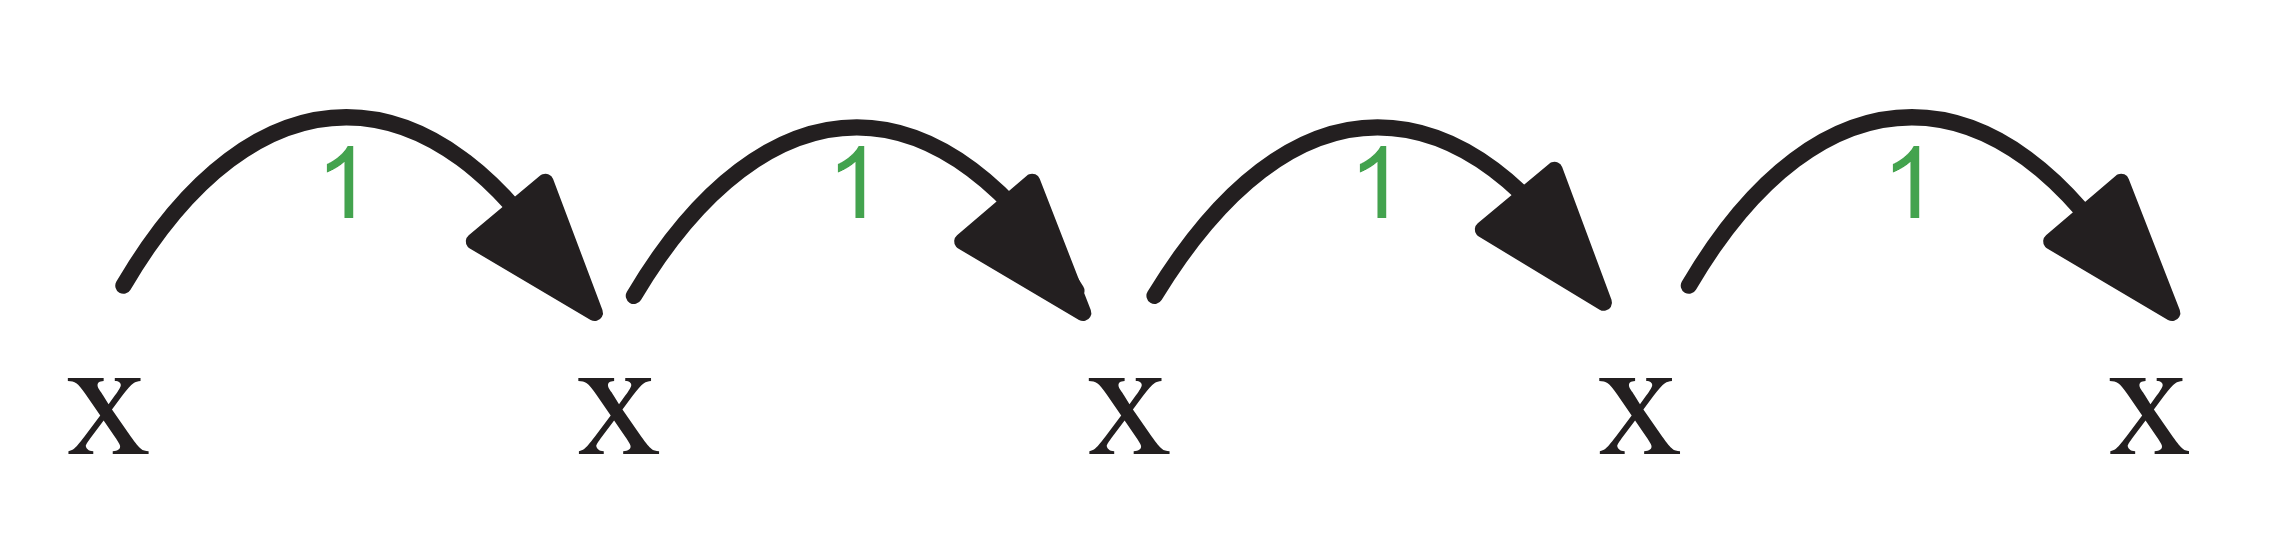
\includegraphics[width=0.5
	\textwidth] {pics/distancesamebranching.png} \caption{Contoh jarak-jarak dependensi konstituen yang berdampingan} 
\label{fig:distancesamebranching} \end{figure}

\begin{figure}
	\centering 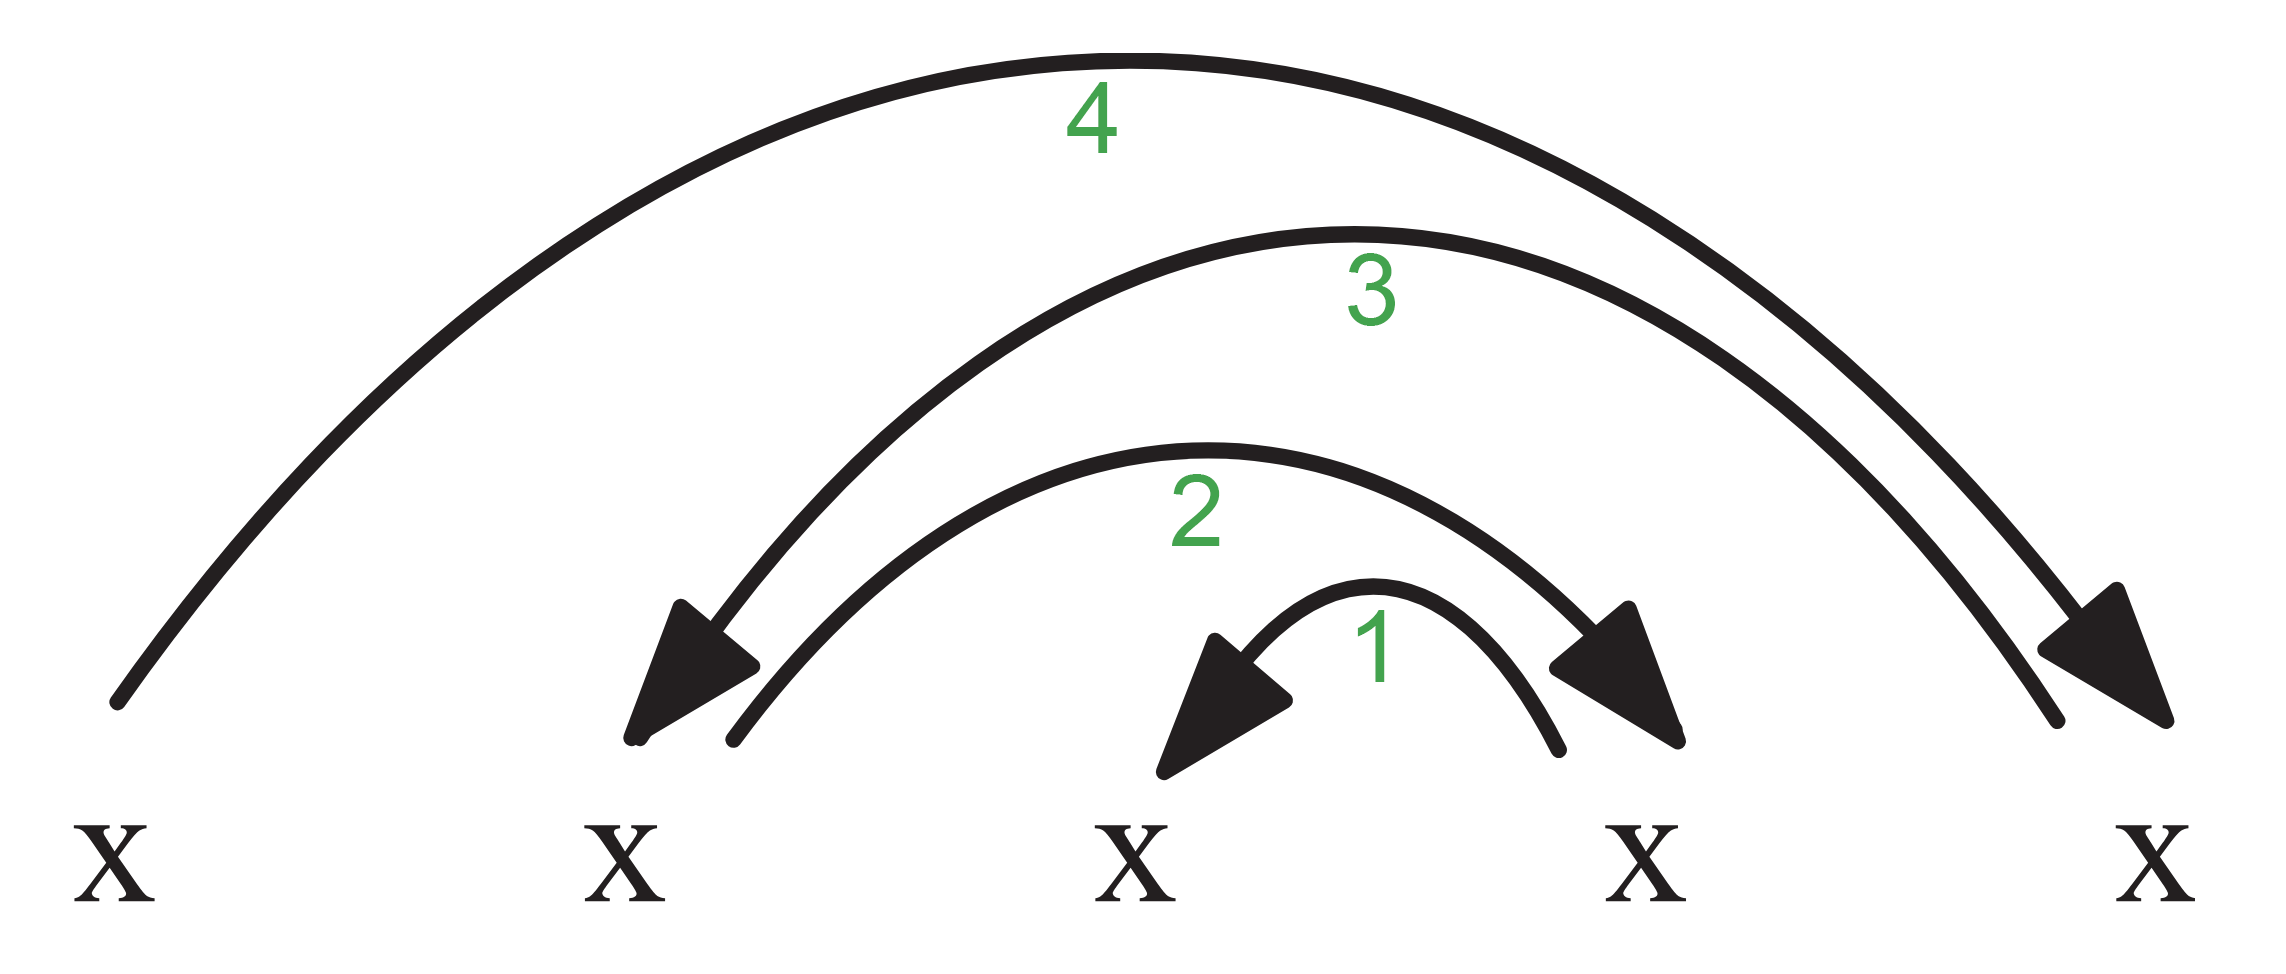
\includegraphics[width=0.5
	\textwidth] {pics/distancemixedbranching.png} \caption{Contoh jarak-jarak dependensi berbagai tautan dependensi} 
\label{fig:distancemixedbranching} \end{figure}

Berdasarkan penelitian terdahulu, terdapat dua pendekatan yang digunakan untuk melihat efisiensi kalimat dari segi dependensi, yaitu dengan menganalisis \textbf{\Gls{panjang-dependensi}} atau \textit{Dependency Length} (DL) dan \textbf{Rata-rata Jarak Dependensi} atau \textit{Mean Dependency Distance} (MDD). \cite{liu2008dependency} dan \cite{liu2017dependency} mengajukan \textbf{Jarak Dependensi} atau \textit{Dependency Distance} (DD) sebagai indikator untuk menghasilkan penghitungan rata-rata jarak dependensi dan telah melakukan penelitian terhadap data lintas bahasa berskala besar. Di sisi lain, panjang dependensi merupakan teori yang dikembangkan salah satunya oleh \cite{gildea2010grammars}, yang seperti \cite{liu2008dependency} dan \cite{liu2017dependency}, merupakan turunan dari kajian-kajian yang sebelumnya dilakukan oleh \citet{gibson1998linguistic, gibson2000dependency} dan \cite{hawkins1994performance}. Penggunaan istilah 'jarak' dan 'panjang' secara prinsip serupa karena keduanya merefleksikan sejauh apa sebuah konstituen terpisahkan dengan konstituen lain tempatnya bergantung atau yang dikendalikannya, tetapi memiliki sedikit perbedaan dalam penghitungan dan aspek dependensi yang ditekankannya. 

%-----------------------------------------------------------------------------%
\subsection{Faktor-faktor yang mempengaruhi tautan dependensi}
%-----------------------------------------------------------------------------%

Penutur sering menggunakan cara yang berbeda untuk menyampaikan pesan dengan makna yang sama \citep{kroch2001syntactic}. Meskipun penelitian ini hanya menitikberatkan pada variasi sintaktis terkait konsep dependensi, perbedaan karakteristik kalimat ini tidak hanya dalam konteks sintaktis, tetapi juga secara fonetis, fonologis, dan perbedaan leksikal. Hubungan produksi kalimat dipandang dari segi sintaktis dengan memori kerja manusia telah beberapa kali dikaji terutama di ruang lingkup psikolinguistik (\citealp{jay2003psychology, levy2013surprisal}) maupun oleh peneliti di bidang ilmu kognitif (\citealp{futrell2015large, christiansen2016now, liu2017dependency}). Hal ini memperlihatkan bahwa konsep dependensi dapat memberikan kontribusi wawasan tidak hanya dari segi linguistik, namun juga secara multidisipliner.

%-----------------------------------------------------------------------------%
\subsubsection{Kognisi manusia dan produksi kalimat}
%-----------------------------------------------------------------------------%
Melalui pendekatan linguistik kuantitatif, beberapa penelitian telah menunjukkan bukti-bukti kecenderungan bahwa semakin jauh panjang dan jarak dependensi, semakin sulit pemrosesan dan analisis struktur sintaktis semakin sulit (\citealp{gibson1998linguistic, hiranuma1999syntactic, jiang2015effects, temperley2007minimization}). Meskipun penelitian ini tidak menelaah aspek kognisi manusia secara mendalam, temuan penelitian ini dapat dikaitkan dengan temuan penelitian-penelitian tersebut dan memberikan wawasan dari aspek linguistik dalam bahasa Indonesia untuk membentuk hipotesis lanjutan secara lintas bahasa.

Panjang dan jarak dependensi antarkonstituen mengindikasikan upaya memori kerja manusia untuk menyimpan secara aktif satu konstituen hingga konstituen lain direalisasikan sehingga maknanya dapat tersampaikan secara utuh (\citealp{hudson2003psychological, liu2008dependency}). Pada penelitian-penelitian terdahulu dalam ruang lingkup ilmu kognitif, memori kerja manusia memiliki batasan (\textit{threshold}) terhadap waktu sehingga proses produksi ataupun pemahaman bahasa tidak bertahan lama dan bersifat sekilas untuk saat itu saja \citep{christiansen2016now}. Oleh karena itu, memori akan bekerja lebih banyak untuk memproduksi ataupun memahami kalimat dengan panjang dan jarak dependensi yang lebih jauh karena kedua indikator tersebut diasumsikan berhubungan linear dengan waktu yang dibutuhkan untuk menyimpan konstituen secara aktif. Dapat dikatakan juga bahwa panjang dan jarak dependensi mengindikasikan tingkat kesulitan sebuah kalimat. 

Dalam penelitian \cite{hiranuma1999syntactic} dan \cite{liu2009chinese}, teks dialog yang diperuntukkan sebagai ujaran lisan memiliki rata-rata jarak dependensi yang berbeda antara teks imajinatif dan teks informatif. Oleh karena itu, \cite{hiranuma1999syntactic} dan \cite{liu2009chinese} beranggapan bahwa teks yang semakin formal (dalam konteks ini adalah bahasa Inggris ragam tulis) memiliki tingkat sintaktis yang lebih sulit. Temuan ini mendasari klasifikasi utama terhadap data penelitian, yaitu ragam tulis dan lisan. \cite{oya2013degree} mendemonstrasikan adanya perbedaan antara jarak dependensi pada teks fiksi dan non-fiksi dalam data bahasa Inggris di mana nilai rata-rata jarak dependensi pada teks fiksi lebih kecil. Namun, \cite{wang2017effects} mengungkapkan bahwa temuan ini dihasilkan tanpa investigasi kemungkinan pengaruh panjang kalimat terhadap jarak dependensi. Hal ini signifikan karena perbedaan rata-rata panjang kalimat antara kedua teks dapat berkontribusi terhadap rata-rata jarak dependensi secara keseluruhan. Kemungkinan adanya pengaruh panjang kalimat terhadap tautan dependensi menjadi dasar klasifikasi data penelitian berdasarkan panjang kalimatnya.

%-----------------------------------------------------------------------------%
\subsubsection{Karakter bahasa dan ketatabahasaan}
%-----------------------------------------------------------------------------%
Beberapa penelitian lain yang menggunakan pendekatan linguistik kuantitatif terhadap korpus data teks telah memulai upaya untuk melihat hubungan panjang dan jarak dependensi dengan tipe bahasa (\citealp{hiranuma1999syntactic, eppler2005syntax, liu2012quantitative}), (\citealp{oya2011syntactic, ferrer2014risks, jiang2015effects}), dan tata bahasa (\citealp{liu2008dependency, gildea2010grammars}). Penelitian-penelitian ini belum menunjukkan konsensus terhadap perbedaan mendasar maupun besar dampak dari pengaruh tersebut terhadap dependensinya. Meskipun demikian, beberapa penelitian ini menjadi pondasi untuk memberikan wawasan dan gambaran secara lintas bahasa mengenai kualitas dependensi yang bersifat universal maupun yang menjadi keunikan bahasa masing-masing. \citet[p. 103]{jiang2015effects} menemukan bahwa distribusi jarak dependensi tidak dipengaruhi oleh tipe bahasa. Meskipun demikian, kedua korpus data menunjukkan karakter yang sama, yaitu trend jarak dependensi yang semakin jauh seiring dengan semakin panjangnya kalimat dan rata-rata jarak dependensi dalam bahasa Mandarin lebih tinggi dibandingkan bahasa Inggris.

Sejauh ini belum ada wawasan linguistik yang dapat memberikan informasi terhadap hal tersebut dengan memanfaatkan data bahasa Indonesia. Bahasa Indonesia memiliki konstruksi kalimat umum SVO atau Subyek-Predikat-Obyek, tetapi memiliki aturan urutan kata yang cukup bebas terkait frasa nomina dan frasa verba \citep{irmawati2015dependency}. \citet[p. 71]{kubler2009dependency} menyatakan bahwa analisis sintaktis berdasarkan teori dependensi dapat membantu memahami hubungan antarkonstituen pada bahasa-bahasa dengan aturan urutan kata yang bebas. Munculnya pertanyaan seberapa besar pengaruh kebebasan urutan konstituen terkait pengurangan jarak dependensi ini juga disebabkan oleh pernyataan dalam penelitian \cite{futrell2015large} yang menyebutkan bahwa temuan dalam bahasa Indonesia menunjukkan hasil pengurangan jarak dependensi yang tertinggi dibandingkan 36 bahasa lain yang diteliti.

%-----------------------------------------------------------------------------%
\section{Efisiensi kalimat dari segi dependensi}
%-----------------------------------------------------------------------------%
Hingga abad ke-20, para linguis mengajukan hipotesis pengurangan jarak Euclidean (\textit{Euclidean distance minimization}) untuk jarak antara konstituen-konstituen kalimat yang bertautan secara sintaktis dan fenomena urutan konstituen lainnya (\citealp{i2004euclidean, ferrer2008some}). Hal ini berkaitan dengan usaha penutur dalam menghasilkan kalimat yang efisien sesuai dengan penelitian yang dilakukan \cite{gildea2015human}. \cite{gildea2015human} menguji hipotesis bahwa penutur cenderung menyusun konstituen dalam kalimat untuk menyampaikan informasi secara efisien dan menemukan bahwa semua bahasa yang menjadi obyek penelitiannya memiliki urutan konstituen yang lebih mudah diproses dan dimengerti. Dalam penelitian tersebut, Gildea dan Jaeger menarik korelasi antara kesaratan informasi dan jarak dependensi dengan menitikberatkan pada urutan konstituen dalam kalimat. Saat ini, istilah \textit{Euclidean distance minimization} digantikan dengan istilah pengurangan memori dalam jaringan atau \textit{online memory minimization} karena para peneliti bahasa melihat korelasi yang signifikan antara pengurangan jarak antarkonstituen dalam sebuah kalimat dengan kemudahan proses memori kerja \citep{ferrer2015placement}. Rata-rata jarak dependensi menjadi ukuran penting dalam memprediksikan tingkat kesulitan atau kemudahan sintaktis ini \citep{hudson1995measuring}. Hipotesis bahwa penutur cenderung mengurangi atau meminimalkan jarak dependensi kemungkinan disebabkan oleh keterbatasan memori kerja manusia yang beradaptasi terhadap faktor tata bahasa (\citealp{i2004euclidean, ferrer2016non, buch2006discontinuous, liu2008dependency, gildea2010grammars, futrell2015large}).

%-----------------------------------------------------------------------------%
\subsection{Kaitan pengurangan panjang dan jarak dependensi dengan proses memori kerja}
%-----------------------------------------------------------------------------%
Beberapa studi berbasis empiris telah dilakukan untuk mengeksplorasi kesulitan pemahaman sebuah bahasa, terutama dalam ranah psikolinguistik dan linguistik kognitif \citep{jay2003psychology}. Pendekatan kuantitatif pada ilmu linguistik dalam penelitian seperti ini terus berkembang hingga saat ini dan penggunaan pendekatan-pendekatan tersebut memberikan kontribusi terhadap akurasi metode linguistik kuantitatif yang dikembangkan. \cite{yngve1960model} merupakan salah satu linguis yang mengajukan konsep jumlah 'simbol' maksimum yang dapat disimpan dalam memori kerja saat mengkonstruksi sebuah kalimat. Hipotesis Kedalaman atau \textit{Depth Hypothesis} yang dikembangkan \cite{yngve1960model} diterjemahkan sebagai konsep untuk menganalisis kesulitan pemahaman sebuah kalimat. Isi hipotesis ini adalah bahwa (a) meskipun semua bahasa memiliki tata bahasa, (b) sebuah kalimat memiliki kedalaman yang tidak melebihi angka tertentu (c) sejumlah atau mendekati jumlah yang merepresentasikan memori kerja cepat dan (d) tata bahasa dari semua bahasa tersebut akan menyertakan metode-metode untuk membatasi konstruksi regresif sehingga kalimat tidak akan melewati batas kedalaman (\citealp{yngve1960model, yngve1996grammar}). Dari hipotesis ini dapat diambil kesimpulan bahwa meskipun tata bahasa memungkinkan adanya kalimat-kalimat yang lebih dalam secara teoretis, dalam prakteknya kedalaman tersebut tidak dapat melewati batas tertentu yang setara dengan kapasitas memori kerja manusia (\citealp{miller1956magical,cowan2001metatheory}). Dengan hipotesis ini, \cite{yngve1960model} mencoba membangun indikator universal untuk kesulitan pemahaman sebuah kalimat. 

\cite{miller1963finitary} mengajukan indikator kompleksitas sintaktis berdasarkan rasio dari simpai akhir dan simpai bukan akhir pada bank pohon struktur sintaktis sebuah kalimat. Pendekatan ini dilanjutkan oleh \cite{frazier1985syntactic} yang menggunakan penghitungan dengan menyesuaikan konteks bahasa lokal untuk mengganti penghitungan global yang bersifat lintas bahasa milik \cite{miller1963finitary} agar indikator tersebut lebih sensitif dan kontekstual. \cite{hawkins1994performance} kemudian muncul dengan asumsi mengenai keterkaitan antara tata bahasa dan urutan kata. Untuk mengukur dan memperkirakan kesulitan sintaktis, Hawkins mengembangkan prinsip Konstituen Terdekat Awal atau \textit{Early Immediate Constituents} (EIC) yang menyatakan bahwa manusia cenderung memilih urutan linear yang memaksimalkan rasio Konstituen Terdekat (IC) terhadap non-IC dalam jangkauan pemahaman ujaran. \cite{hawkins2004efficiency} memperbaharui EIC menjadi Meminimalkan Jangkauan atau \textit{Minimize Domain} (MiD) dengan memanfaatkan teori dependensi. Prinsip ini menyatakan bahwa manusia cenderung meminimalkan deret unit linguistik yang memiliki relasi semantis dan/atau meminimalkan proses dependensi yang terlibat \citep[pp. 44-48]{hawkins2004efficiency}. Prinsip ini secara langsung memperlihatkan keterkaitan antara urutan linear konstituen linear dengan pengolahan bahasa yang dilakukan dalam memori kerja manusia.

Hipotesis yang muncul dari penelitian-penelitian tersebut menggambarkan ketertarikan dunia linguistik atas indikator kompleksitas kalimat yang melibatkan hubungan antara urutan linear konstituen, kesulitan sintaktis serta bagaimana dependensi antarunit linguistik berperan di dalam konteks indikator kompleksitas tersebut. Penekanan dependensi dalam area penelitian ini adalah jika struktur kognitif manusia berbentuk seperti jejaring \citep{hudson2007language}, analisis terhadap jejaring dependensi sintaktis juga merupakan langkah penting menuju pemetaan jejaring kognitif konseptual yang secara langsung menggambarkan kerja kognisi manusia \citep{liu2008dependency}. \cite{liu2008dependency} menyimpulkan bahwa dibandingkan dengan struktur frasa, keterkaitan struktur dependensi dengan struktur kognitif dan jejaring bahasa, memiliki hubungan yang lebih dekat. Terdapat kesamaan dalam prinsip-prinsip dari berbagai penelitian tersebut, yaitu indikasi bahwa konstituen-konstituen yang memiliki relasi semantik cenderung akan berdekatan dalam kalimat. 

\cite{liu2017dependency} mengembangkan proposal indikator yang menggunakan jarak dependensi menjadi hipotesis \textbf{Pengurangan Jarak Dependensi} atau \textit{Dependency Distance Minimization} (yang selanjutnya akan disingkat menjadi DDM). Sebagai contoh, istilah 'jarak' sering digunakan jika seseorang bergerak menuju sebuah tempat hingga orang tersebut berhenti. Dalam proses produksi dan pemahaman bahasa, 'jarak' dependensi baru akan dapat terukur apabila dependensi kedua konstituen telah terbentuk (konstituen kedua sudah diujarkan, dibaca, ditulis, atau didengar). \citet[p. 3]{liu2017dependency} berargumen bahwa 'panjang' merefleksikan ukuran dengan karakteristik statis dari sebuah entitas dan 'jarak' lebih menggambarkan proses dinamis sehingga dalam konteks dependensi sebuah kalimat, para peneliti tersebut beranggapan istilah 'jarak' lebih tepat digunakan. Untuk mendapatkan gambaran DDM, Liu (\citealp{liu2008dependency, liu2017dependency}) menjabarkan rumus untuk menghitung \textbf{Rata-rata Jarak Dependensi}. \cite{hudson2010introduction} dan \cite{i2004euclidean} menggunakan pendekatan yang kurang lebih sama untuk menghitung MDD dalam sebuah kalimat. Dalam studinya, \cite{i2004patterns} melakukan kajian untuk memperlihatkan bahwa jejaring sintaksis merupakan contoh 'dunia-dunia kecil' yang berarti angka rata-rata dari tautan dalam simpai ditemukan sangat kecil. Hipotesis utama DDM dijabarkan Liu (\citealp{liu2008dependency, liu2017dependency}) sebagai berikut:

\begin{itemize}
\item Manusia cenderung memilih urutan konstituen yang dapat mengurangi rata-rata jarak dependensi.
\item Terdapat batasan rata-rata jarak dependensi pada hampir semua kalimat dalam bahasa manusia.
\item Tata bahasa dan kognisi manusia bekerja sama untuk menekan jarak dependensi agar berada di dalam batasan tersebut.
\end{itemize}

Dalam penelitian lintas bahasa berskala besar lain, \cite{futrell2015large} menggunakan hipotesis \textbf{Pengurangan Panjang Dependensi} atau \textit{Dependency Length Minimization} (yang selanjutkan akan disingkat menjadi DLM). Penelitian lintas bahas ini memanfaatkan korpus data sebanyak 37 bahasa, termasuk bahasa Indonesia. Hipotesis ini sebelumnya muncul dalam penelitian Temperley dan Gildea (\citealp{temperley2007minimization, temperley2008dependency, gildea2010grammars}). \cite{gildea2010grammars} menggunakan istilah 'panjang' dalam DLM karena menitikberatkan pada kompleksitas keseluruhan kalimat. Penghitungan yang digunakan untuk melihat indikasi DLM didapatkan dengan menjumlahkan keseluruhan jarak tautan-tautan dependensi dalam sebuah kalimat seperti yang terlihat pada Gambar 1.1 di Bab 1. \cite{liu2017dependency} dan \cite{i2004euclidean} beranggapan bahwa pendekatan ini cukup sensitif terhadap panjang kalimat atau kalimat sehingga perbedaan rata-rata yang muncul kurang bisa mewakili kesulitan sintaktis karena ada kecenderungan bahwa kalimat yang semakin panjang akan menghasilkan angka lebih besar. Hipotesis utama dari DLM dijabarkan oleh \cite{gildea2010grammars} serta \cite{futrell2015large} sebagai prinsip bahasa yang telah banyak diakui mengenai preferensi penutur untuk mendekatkan konstituen-konstituen yang memiliki relasi semantis dalam sebuah kalimat.

%-----------------------------------------------------------------------------%
\subsection{Kecenderungan posisi induk terhadap konstituen terikat dalam kalimat}
%-----------------------------------------------------------------------------%

Dalam studi-studi termutakhir, urutan kata direfleksikan juga melalui arah dependensi \citep{hudson2007language}. Arah dependensi ini mengindikasikan apakah tautan dependensi diawali atau diakhiri oleh induk. Posisi induk yang menentukan tautan dependensi dengan konstituen terikatnya ini dikenal juga dengan istilah \textbf{\gls{direksionalitas-induk}} atau \textit{head directionality}. Sebagai contoh, \cite{hudson2003psychological} mengungkapkan bahwa bahasa Jepang merupakan salah satu bahasa yang bentuk relasi dependensinya cenderung diakhiri oleh induk. Konsep penghitungan panjang dan jarak dependensi ini berkaitan dengan logika kesulitan pengolahan dalam memori kerja \citep{hudson2007language}. \cite{hudson2007language} menjelaskan bahwa dalam menghasilkan kalimat yang berisi setidaknya dua konstituen, kedua konstituen tersebut akan tersimpan secara aktif di dalam memori kerja hingga dependensi di antara keduanya terbentuk. Hal ini berarti bahwa jarak dependensi diasumsikan dapat merepresentasikan waktu atau usaha yang dibutuhkan untuk menyimpan konstituen pertama dan kedua dalam memori kerja hingga konstituen kedua selesai diproses (diujarkan, didengar, dibaca, atau ditulis). Dari konsep ini muncul hipotesis bahwa jarak dependensi yang semakin jauh menuntut usaha pengolahan dalam memori kerja yang semakin berat (\citealp{hudson2007language, gibson1998linguistic}).

Semua bahasa, baik yang memiliki urutan kata bebas ataupun urutan kata tetap, memiliki kaidah urutan tertentu yang menentukan urutan linear konstituen-konstituen dalam sebuah kalimat \citep{tesniere1959elements}. Hal ini berarti hierarki relasi antarkonstituen, dalam konteks dependensi, memiliki korelasi dengan arah secara linear \citep{greenberg1963some}. Terdapat perbedaan mengenai urutan linear antarkonstituen antara yang dibahas oleh \cite{tesniere1959elements} dengan \cite{greenberg1963some}. Dalam hal ini, \cite{greenberg1963some} lebih menekankan pada relasi gramatikal dalam sebuah kalimat, sedangkan \cite{tesniere1959elements} berupaya untuk membangun analisis menyeluruh terhadap sebuah kalimat berdasarkan relasi gramatikal tersebut. Penggunaan istilah "cenderung" atau "kecenderungan" (\textit{pr{\'e}f{\'e}rence} dalam bahasa Perancis) digunakan \cite{tesniere1959elements} untuk mengklasifikasikan bahasa berdasarkan direksionalitas induknya.

Hingga saat ini, belum ada konvensi mengenai direksionalitas induk terkait hierarki dan pengolahan dalam memori kerja. Namun, beberapa studi telah dilakukan untuk memberikan penjelasan tambahan mengenai penerapan aturan tata bahasa. Beberapa penelitian pada awal berkembangnya teori dependensi, menemukan bahwa sebuah bahasa cenderung menerapkan arah relasi yang konsisten, baik itu \gls{diawali-induk} (\textit{head-first} atau \textit{head-initial}) maupun \gls{diakhiri-induk} (\textit{head-last} atau \textit{head-final})\footnote{Seperti yang dijelaskan sebelumnya, induk (\textit{head}) di sini sedikit berbeda dengan kepala (\textit{head}) pada teori struktur frasa. Sehingga, bentuk relasi dependensi diawali atau diakhiri induk yang dibahas pada bagian ini terbatas hanya pada penerapannya berdasarkan teori dependensi dan bukan struktur frasa.} (\citealp{hawkins1994performance, radford1997syntactic, vennemann1994linguistic}). Tindakan yang konsisten ini juga diasumsikan sebagai penerapan tata bahasa sebagai strategi untuk meminimalkan jarak antara induk dan konstituen terikatnya (\citealp{hawkins1994performance, frazier1985syntactic}). \cite{liu2010dependency} juga telah berupaya untuk memberikan validitas berdasarkan data mengenai arah dependensi dan kaitannya dengan klasifikasi topologis sebuah bahasa.

\begin{figure}
	\centering 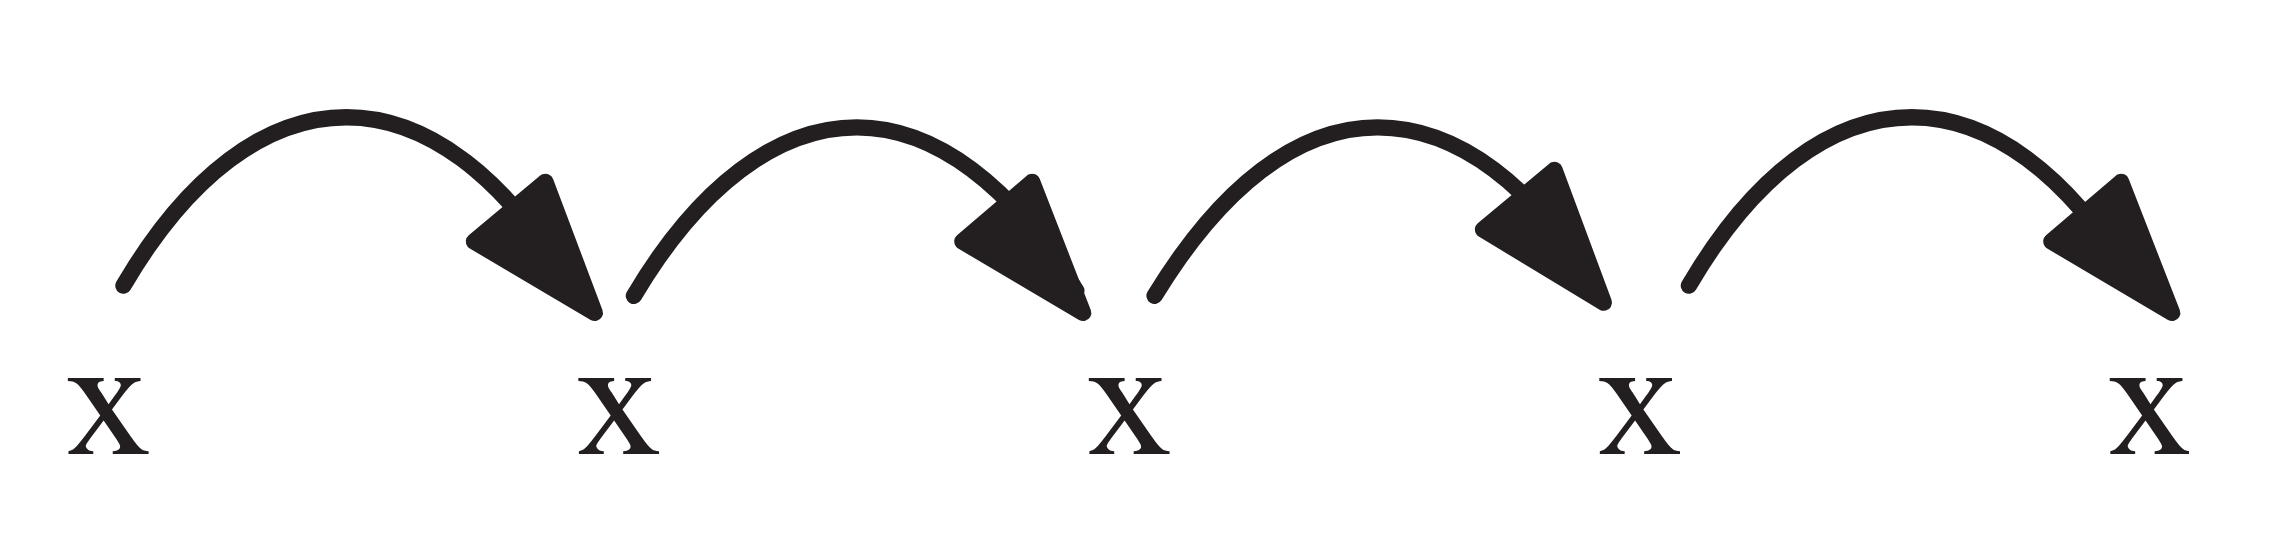
\includegraphics[width=0.5
	\textwidth] {pics/samebranching.png} \caption{\Gls{percabangan-searah} atau \textit{same-branching}} 
\label{fig:samebranching} \end{figure}

\begin{figure}
	\centering 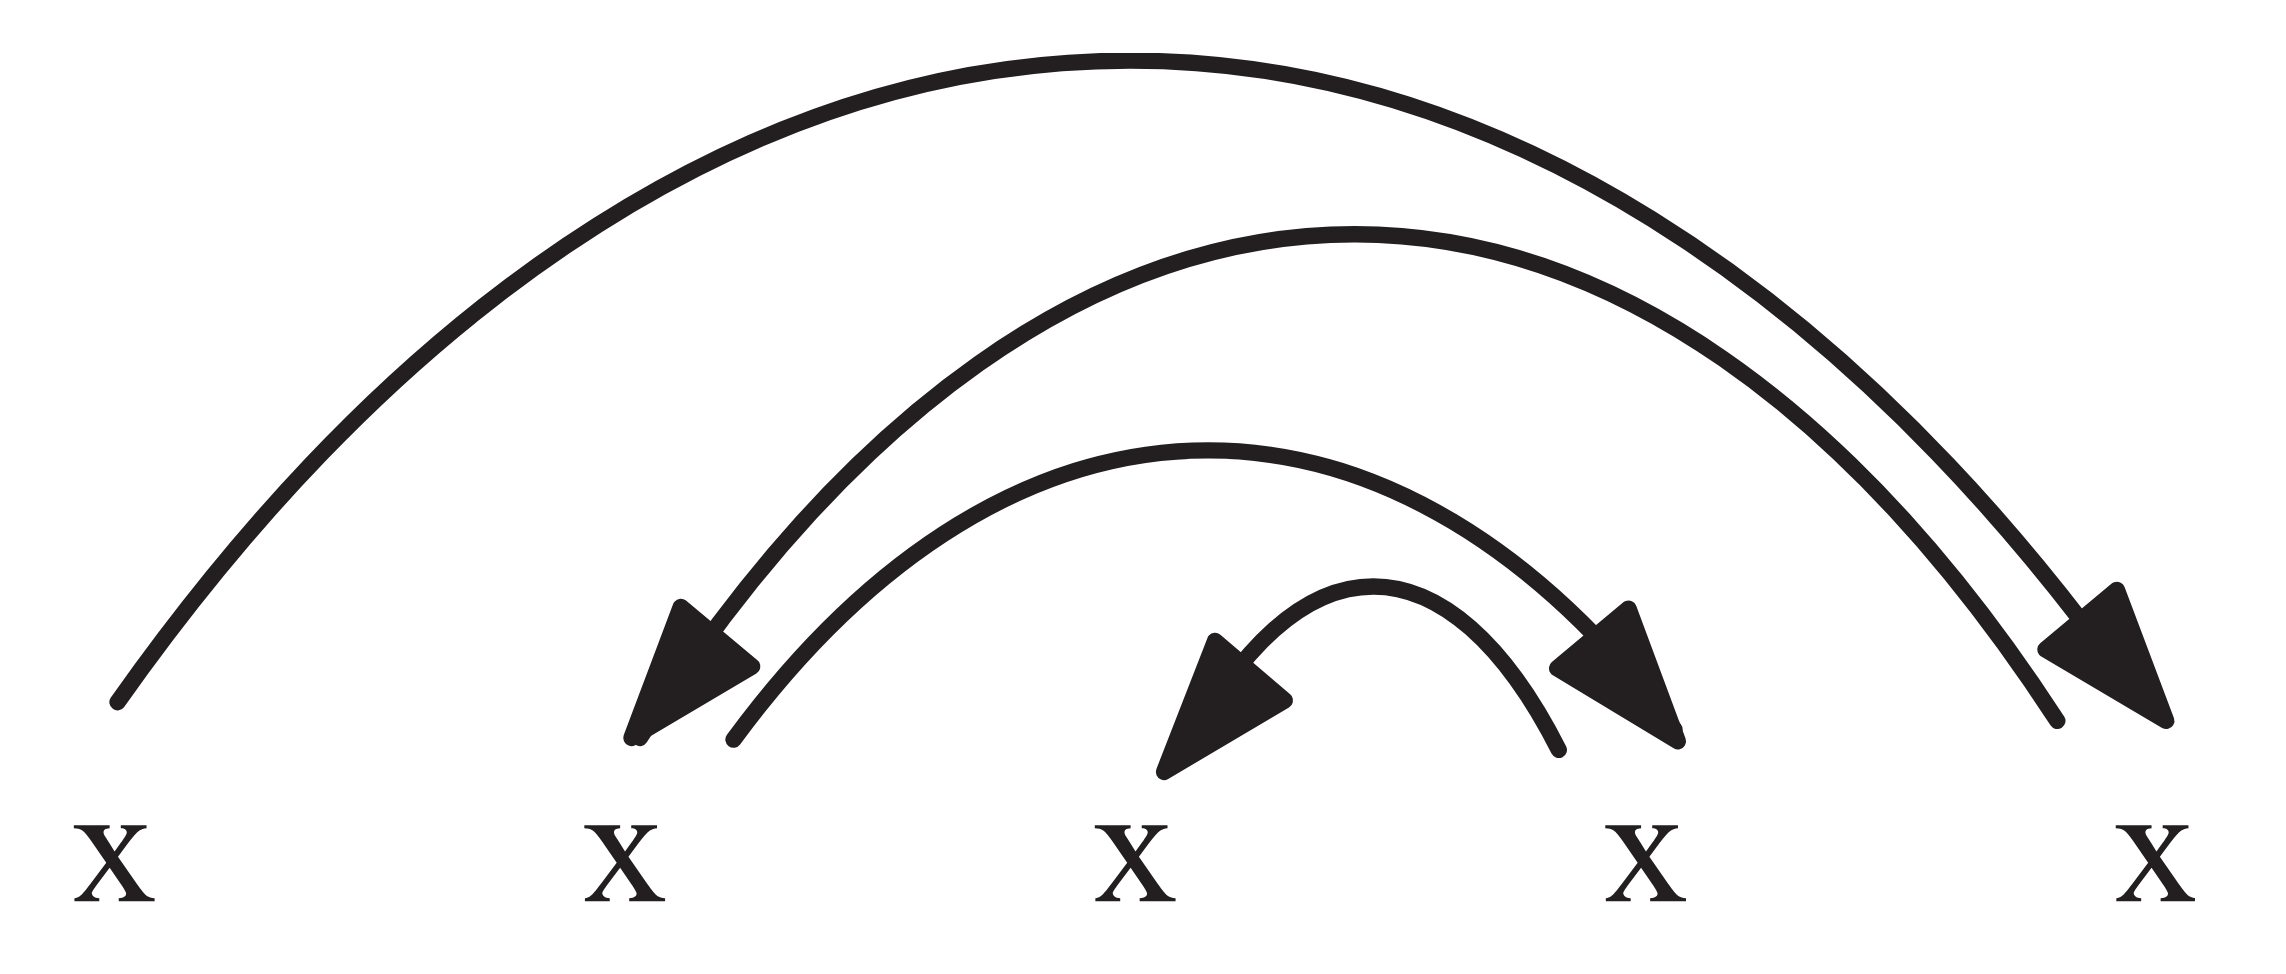
\includegraphics[width=0.5
	\textwidth] {pics/mixedbranching.png} \caption{\Gls{percabangan-beda-arah} atau \textit{mixed-branching}} 
\label{fig:mixedbranching} \end{figure}

Perbandingan percabangan pada \pic~\ref{fig:samebranching} dan \pic~\ref{fig:mixedbranching} mengilustrasikan tautan-tautan yang dibentuk oleh masing-masing tipe percabangan. Percabangan searah atau \textit{same branching} dengan satu relasi yang berkelanjutan tidak mungkin akan secara konsisten terjadi, terutama pada kalimat yang lebih panjang sehingga asumsi ini dipertanyakan oleh \cite{temperley2008dependency} yang menganggap bahwa percabangan searah ini tidak selalu optimal dalam menggambarkan penampilan bahasa. \cite{temperley2008dependency} meneruskan asumsi ini berdasarkan penelitian \cite{dryer1992greenbergian} terhadap 625 bahasa yang mengungkapkan bahwa percabangan searah yang konvensional tidak dapat menggambarkan dengan baik aplikasi tata bahasa pada tuturan nyata dalam studi penampilan bahasa. \cite{dryer1992greenbergian} menggambarkan karakter tata bahasa mengenai hal ini sebagai berikut: frasa yang mengandung banyak konstituen cenderung memiliki percabangan searah, sedangkan arah dependensi frasa yang hanya mengandung satu konstituen ditemukan tidak konsisten. Kajian \cite{dryer1992greenbergian} yang dikutip dalam \cite{gildea2010grammars} memperlihatkan dengan bukti empiris adanya gabungan percabangan searah dan percabangan beda arah (\textit{mixed branching}) untuk menghasilkan keseimbangan antara arah dependensi positif (diawali induk) dan dependensi negatif (diakhiri induk) dalam mendapatkan nilai panjang dependensi terkecil (\pic~\ref{fig:balancedbranching}).

\begin{figure}
	\centering 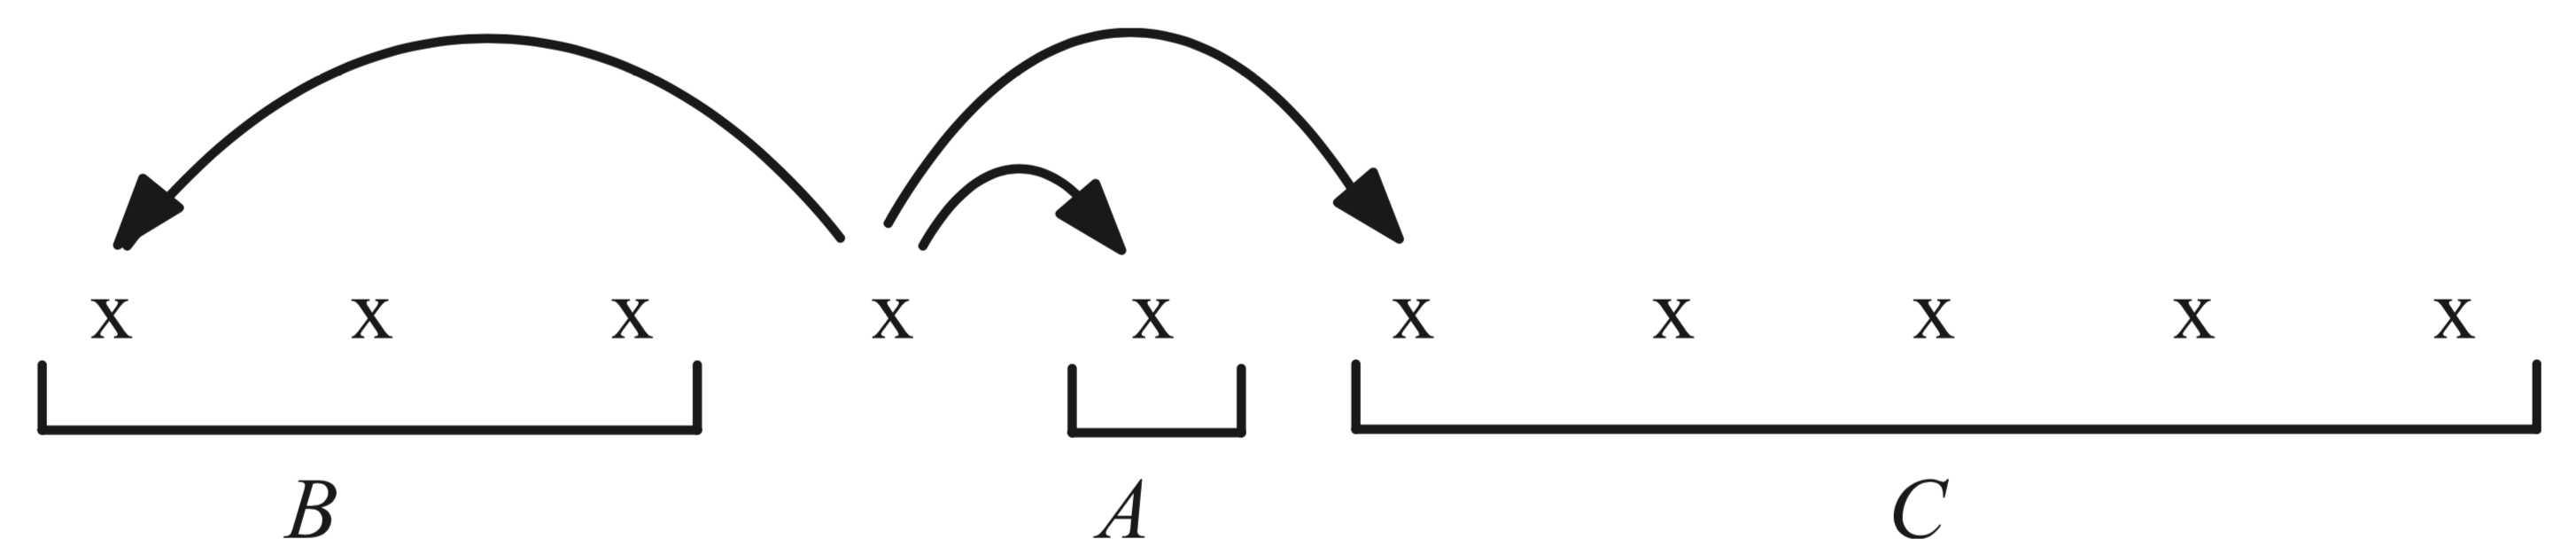
\includegraphics[width=0.8
	\textwidth] {pics/balancedbranching.png} \caption{Keseimbangan direksionalitas induk} 
\label{fig:balancedbranching} \end{figure}

%-----------------------------------------------------------------------------%
\subsection{Perubahan valensi akar verbal}
%-----------------------------------------------------------------------------%
Penjabaran konsep dependensi juga mencakup seberapa kuat sebuah konstituen mengikat konstituen lain dalam kalimat. Dalam teori dependensi \citep[p. 239]{tesniere1959elements} dan \textit{Word Grammar} \citep[p. 165]{hudson2007language}, kemampuan sebuah induk (sebagai contoh: verba) menarik konstituen di sekitarnya (sebagai contoh: aktor pelaku yang umumnya adalah nomina) disebut dengan \textbf{valensi}. Sebagai ilustrasi, agar penerapan konstituen \textit{memandangi} dalam kalimat menjadi gramatikal, konstituen tersebut (yang memiliki fungsi sebagai proses) menuntut keterlibatan dua konstituen lain seperti pada kalimat: $Budi_1$ $memandangi$ $lukisan_2$. Verba \textit{memandangi} mengalokasikan fungsi \textit{Budi} sebagai \textit{yang memandangi} (aktor pelaku atau \textit{agent}) pada posisi pertama, dan \textit{lukisan} sebagai \textit{yang dipandangi} (obyek penderita atau \textit{patient}) \citep{welke2002deutsche}. Kebutuhan fungsional verba tersebut menentukan kategori dan posisi yang harus diisi agar sebuah kalimat menjadi gramatikal. Tidak hanya pelengkap, verba juga dapat berkombinasi dengan keterangan (\textit{adjunct}) seperti pada kalimat: $Budi_1$ $memandangi$ $lukisan_2$ $di$ $museum_3$. Pelengkap juga dapat bersifat tidak wajib seperti pada contoh $dia_1$ $membaca$ $buku_2$ dan $dia_1$ $membaca$. Konstituen \textit{buku} merupakan obyek penderita langsung yang tidak wajib muncul agar pendengar memahami proses \textit{membaca}. 

Hingga saat ini, belum ada pendekatan linguistik kuantitatif ataupun perangkat komputasional dan inventori leksikon valensi untuk bahasa Indonesia. Oleh karena itu, analisis valensi dalam penelitian ini dilakukan secara manual atau bersifat kualitatif dengan menggunakan referensi dari anotasi yang ada. Analisis valensi dalam penelitian ini mengambil obyek berupa akar verbal pada simpai pusat karena diduga merupakan bentuk rangka valensi yang paling umum. Perlu ditekankan bahwa analisis valensi ini tidak ditujukan untuk mengidentifikasi kalimat yang bersifat gramatikal dan tidak gramatikal, namun menitikberatkan pada fenomena linguistik yang muncul dalam tuturan nyata sesuai dengan korpus data yang dikumpulkan. Meskipun kemunculan akar verbal pada simpai pusat diduga memiliki frekuensi tertinggi, beberapa nomina dan adjektiva juga dapat muncul pada simpai pusat dan memiliki valensi tertentu (\citealp{vreznivckova2003czech, hajic2003pdt}).
